\chapter{Farmer-Wolf-Goat-Cabbage Models}\label{app:fwgc}
This appendix contains IOGGs and IOSTSs for the Farmer-Wolf-Goat-Cabbage puzzle. This puzzle is explained in section~\ref{sec:fwgc}. The IOGG for the puzzle is in Figures~\ref{fig:gg-fwgc} and ~\ref{fig:gg-fwgc-continued}, the extended IOGG for the puzzle is in Figure~\ref{fig:gg-fwgc-extended}, the IOSTS for the puzzle is in Figure~\ref{fig:sts-fwgc} and the extended IOSTS is in Figure~\ref{fig:sts-fwgc-extended}. 

  \begin{figure}[ht]
  \begin{center}
    \subfloat[The initial graph]{\label{fig:start-fwgc}% To use this figure in your LaTeX document
% import the package groove/resources/groove2tikz.sty
%
% Special colors
\begin{tikzpicture}[
% Special color styles
scale=\tikzscale]
\node[node] (n8)  at (2.350, -0.680) {\ml{right}};
\node[node] (n3)  at (0.545, -1.010) {\ml{wolf}};
\node[node] (n4)  at (0.570, -1.370) {\ml{goat}};
\node[node] (n1)  at (2.355, -1.230) {\ml{bank}};
\node[node] (n5)  at (0.670, -1.730) {\ml{cabbage}};
\node[node] (n0)  at (1.555, -1.220) {\ml{bank}};
\node[node] (n7)  at (1.565, -0.680) {\ml{left}};
\node[node] (n2)  at (0.635, -0.680) {\ml{farmer}};
\path[edge] (n2)  -- node[lab]{at} (n0) ;
\path[edge] (n5)  -- node[lab]{at} (n0) ;
\path[edge] (n4)  -- node[lab]{at} (n0) ;
\path[edge](n1.north -| 2.350, -0.680) -- node[lab]{side} (n8) ;
\path[edge](n0.north -| 1.565, -0.680) -- node[lab]{side} (n7) ;
\path[edge] (n3)  -- node[lab]{at} (n0) ;
\userdefinedmacro
\end{tikzpicture}
\renewcommand{\userdefinedmacro}{\relax}
}\hspace{20px}
    \subfloat[?n (priority 0)]{\label{fig:n-fwgc}% To use this figure in your LaTeX document
% import the package groove/resources/groove2tikz.sty
%
% Special colors
\begin{tikzpicture}[
% Special color styles
scale=\tikzscale]
\node[node] (n2)  at (2.015, -2.045) {\ml{farmer}};
\node[node] (n1)  at (2.045, -0.885) {\ml{bank}};
\node[node] (n0)  at (0.925, -2.035) {\ml{bank}};
\path[edge, -] (n0)  -- node[lab]{\textit{!=}} (n1) ;
\path[deledge](n2.west |- 0.925, -2.035) -- node[dellab]{at} (n0) ;
\path[newedge](n2.north -| 2.045, -0.885) -- node[newlab]{at} (n1) ;
\userdefinedmacro
\end{tikzpicture}
\renewcommand{\userdefinedmacro}{\relax}
} \\
    \subfloat[?w valid (priority 0)]{\label{fig:w-fwgc}% To use this figure in your LaTeX document
% import the package groove/resources/groove2tikz.sty
%
% Special colors
\begin{tikzpicture}[
% Special color styles
scale=\tikzscale]
\node[node] (n4)  at (2.305, -1.560) {\ml{wolf}};
\node[node] (n3)  at (1.745, -1.080) {\ml{farmer}};
\node[node] (n0)  at (0.955, -1.570) {\ml{bank}};
\node[node] (n1)  at (2.355, -0.560) {\ml{bank}};
\node[node] (n2)  at (0.920, -0.560){};
\path[newedge] (n3)  -- node[newlab]{at} (n1) ;
\path[deledge] (n3)  -- node[dellab]{at} (n0) ;
\path[nacedge](n1.west |- 0.920, -0.560) -- node[naclab]{side} (n2) ;
\path[edge](n0.north -| 0.920, -0.560) -- node[lab]{side} (n2) ;
\path[deledge](n4.west |- 0.955, -1.570) -- node[dellab]{at} (n0) ;
\path[newedge](n4.north -| 2.355, -0.560) -- node[newlab]{at} (n1) ;
\userdefinedmacro
\end{tikzpicture}
\renewcommand{\userdefinedmacro}{\relax}
}\hspace{20px}
    \subfloat[?w invalid (priority 0)]{\label{fig:w-invalid-fwgc}% To use this figure in your LaTeX document
% import the package groove/resources/groove2tikz.sty
%
% Special colors
\begin{tikzpicture}[
% Special color styles
scale=\tikzscale]
\node[node] (n0)  at (2.065, -1.515) {\ml{bank}};
\node[node] (n1)  at (1.015, -1.525) {\ml{bank}};
\node[node] (n4)  at (2.085, -1.025) {\ml{wolf}};
\node[node] (n3)  at (1.025, -1.005) {\ml{farmer}};
\node[newnode] (n5)  at (3.315, -1.515) {\ml{\textbf{InvalidMove}}};
\path[edge](n3.south -| 1.015, -1.525) --  (n1) ;
\node[lab] at (1.015, -1.265){at};
\path[edge](n4.south -| 2.065, -1.515) -- node[lab]{at} (n0) ;
\path[edge, -](n1.east |- 2.065, -1.515) -- node[lab]{\textit{!=}} (n0) ;
\userdefinedmacro
\end{tikzpicture}
\renewcommand{\userdefinedmacro}{\relax}
} \\
    \subfloat[?g valid (priority 0)]{\label{fig:g-fwgc}% To use this figure in your LaTeX document
% import the package groove/resources/groove2tikz.sty
%
% Special colors
\begin{tikzpicture}[
% Special color styles
scale=\tikzscale]
\node[node] (n2)  at (2.285, -0.915) {\ml{farmer}};
\node[node] (n1)  at (2.275, -2.205) {\ml{bank}};
\node[node] (n0)  at (0.855, -0.925) {\ml{bank}};
\node[node] (n3)  at (1.865, -1.275) {\ml{goat}};
\path[edge, -] (n0)  -- node[lab]{\textit{!=}} (n1) ;
\path[newedge] (n3)  -- node[newlab]{at} (n1) ;
\path[deledge] (n3)  -- node[dellab]{at} (n0) ;
\path[deledge](n2.west |- 0.855, -0.925) -- node[dellab]{at} (n0) ;
\path[newedge](n2.south -| 2.275, -2.205) -- node[newlab]{at} (n1) ;
\userdefinedmacro
\end{tikzpicture}
\renewcommand{\userdefinedmacro}{\relax}
}\hspace{20px}
    \subfloat[?g invalid (priority 0)]{\label{fig:g-invalid-fwgc}% To use this figure in your LaTeX document
% import the package groove/resources/groove2tikz.sty
%
% Special colors
\begin{tikzpicture}[
% Special color styles
scale=\tikzscale]
\node[newnode] (n5)  at (3.315, -1.515) {\ml{\textbf{InvalidMove}}};
\node[node] (n3)  at (1.025, -1.005) {\ml{farmer}};
\node[node] (n4)  at (2.085, -1.025) {\ml{goat}};
\node[node] (n1)  at (1.015, -1.525) {\ml{bank}};
\node[node] (n0)  at (2.065, -1.515) {\ml{bank}};
\path[edge](n3.south -| 1.015, -1.525) --  (n1) ;
\node[lab] at (1.015, -1.265){at};
\path[edge](n4.south -| 2.065, -1.515) -- node[lab]{at} (n0) ;
\path[edge, -](n1.east |- 2.065, -1.515) -- node[lab]{\textit{!=}} (n0) ;
\userdefinedmacro
\end{tikzpicture}
\renewcommand{\userdefinedmacro}{\relax}
} \\
    \subfloat[?c valid (priority 0)]{\label{fig:c-fwgc}% To use this figure in your LaTeX document
% import the package groove/resources/groove2tikz.sty
%
% Special colors
\begin{tikzpicture}[
% Special color styles
scale=\tikzscale]
\node[node] (n1)  at (2.495, -1.015) {\ml{bank}};
\node[node] (n0)  at (0.945, -2.365) {\ml{bank}};
\node[node] (n3)  at (1.985, -1.975) {\ml{farmer}};
\node[node] (n4)  at (2.455, -2.365) {\ml{cabbage}};
\path[deledge](n4.west |- 0.945, -2.365) -- node[dellab]{at} (n0) ;
\path[deledge] (n3)  -- node[dellab]{at} (n0) ;
\path[newedge] (n3)  --  (n1) ;
\node[newlab] at (2.063, -1.303){at};
\path[newedge](n4.north -| 2.495, -1.015) -- node[newlab]{at} (n1) ;
\path[edge, -] (n0)  -- node[lab]{\textit{!=}} (n1) ;
\userdefinedmacro
\end{tikzpicture}
\renewcommand{\userdefinedmacro}{\relax}
}\hspace{20px}
    \subfloat[?c invalid (priority 0)]{\label{fig:c-invalid-fwgc}% To use this figure in your LaTeX document
% import the package groove/resources/groove2tikz.sty
%
% Special colors
\begin{tikzpicture}[
% Special color styles
scale=\tikzscale]
\node[newnode] (n5)  at (3.315, -1.515) {\ml{\textbf{InvalidMove}}};
\node[node] (n3)  at (1.025, -1.005) {\ml{farmer}};
\node[node] (n4)  at (2.085, -1.025) {\ml{cabbage}};
\node[node] (n1)  at (1.015, -1.525) {\ml{bank}};
\node[node] (n0)  at (2.065, -1.515) {\ml{bank}};
\path[edge](n3.south -| 1.015, -1.525) --  (n1) ;
\node[lab] at (1.020, -1.270){at};
\path[edge](n4.south -| 2.065, -1.515) -- node[lab]{at} (n0) ;
\path[edge, -](n1.east |- 2.065, -1.515) -- node[lab]{\textit{!=}} (n0) ;
\userdefinedmacro
\end{tikzpicture}
\renewcommand{\userdefinedmacro}{\relax}
} \\
  \end{center}
  \caption{The IOGG of the farmer-wolf-goat-cabbage puzzle}
  \label{fig:gg-fwgc}
  \end{figure}

  \begin{figure}[ht]
  \setcounter{subfigure}{8}
  \begin{center}
    \subfloat[!retry (priority 1)]{\label{fig:retry-fwgc}\parbox{4cm}{\centering% To use this figure in your LaTeX document
% import the package groove/resources/groove2tikz.sty
%
% Special colors
\begin{tikzpicture}[
% Special color styles
scale=\tikzscale]
\node[delnode] (n0)  at (1.155, -0.905) {\ml{\textbf{InvalidMove}}};
\userdefinedmacro
\end{tikzpicture}
\renewcommand{\userdefinedmacro}{\relax}
}}\\
    \subfloat[!eaten (priority 1)]{\label{fig:reinit}% To use this figure in your LaTeX document
% import the package groove/resources/groove2tikz.sty
%
% Special colors
\begin{tikzpicture}[
% Special color styles
scale=\tikzscale]
\node[node] (n14)  at (4.815, -0.505) {\ml{bank}};
\node[node] (n17)  at (4.815, -1.945) {\ml{bank}};
\node[node] (n10)  at (3.795, -0.495) {\ml{farmer}};
\node[node] (n11)  at (3.750, -0.955) {\ml{wolf}};
\node[node] (n16)  at (4.755, -1.395) {\ml{bank}};
\node[node] (n8)  at (2.665, -1.180) {\ml{\textit{left}\\bank}};
\node[node] (n13)  at (3.815, -1.945) {\ml{cabbage}};
\node[node] (n5)  at (1.805, -1.165){};
\node[node] (n0)  at (1.805, -1.815) {\ml{farmer}};
\node[node] (n15)  at (4.825, -0.965) {\ml{bank}};
\node[node] (n1)  at (0.795, -1.815) {\ml{bank}};
\node[node] (n4)  at (0.795, -0.555){};
\node[node] (n3)  at (0.775, -1.175) {\ml{bank}};
\node[node] (n12)  at (3.715, -1.405) {\ml{goat}};
\path[edge](n4.south -| 0.775, -1.175) -- node[lab]{at} (n3) ;
\path[edge, -](n1.north -| 0.775, -1.175) -- node[lab]{\textit{!=}} (n3) ;
\path[deledge](n11.east |- 4.825, -0.965) -- node[dellab]{at} (n15) ;
\path[newedge] (n11)  -- node[newlab]{at}(n8.east |- 3.750, -0.955);
\path[deledge](n12.east |- 4.755, -1.395) -- node[dellab]{at} (n16) ;
\path[edge](n0.west |- 0.795, -1.815) -- node[lab]{at} (n1) ;
\path[newedge] (n13)  -- node[newlab]{at} (n8) ;
\path[deledge](n13.east |- 4.815, -1.945) -- node[dellab]{at} (n17) ;
\path[edge](n5.west |- 0.775, -1.175) -- node[lab]{at} (n3) ;
\path[newedge] (n10)  -- node[newlab]{at} (n8) ;
\path[deledge](n10.east |- 4.815, -0.505) -- node[dellab]{at} (n14) ;
\path[newedge] (n12)  -- node[newlab]{at}(n8.east |- 3.715, -1.405);
\path[edge] (n4)  -- node[lab]{eats} (n5) ;
\userdefinedmacro
\end{tikzpicture}
\renewcommand{\userdefinedmacro}{\relax}
}\\
    \subfloat[!done (priority 1)]{\label{fig:done}% To use this figure in your LaTeX document
% import the package groove/resources/groove2tikz.sty
%
% Special colors
\begin{tikzpicture}[
% Special color styles
scale=\tikzscale]
\node[node] (n2)  at (2.615, -2.685) {\ml{goat}};
\node[node] (n7)  at (1.305, -2.500) {\ml{\textit{left}\\bank}};
\node[node] (n0)  at (2.725, -1.915) {\ml{farmer}};
\node[node] (n1)  at (2.610, -2.295) {\ml{wolf}};
\node[node] (n4)  at (3.915, -2.475) {\ml{\textit{right}\\bank}};
\node[node] (n3)  at (2.755, -3.125) {\ml{cabbage}};
\path[newedge] (n1)  -- node[newlab]{at}(n7.east |- 2.610, -2.295);
\path[deledge] (n2)  -- node[dellab]{at}(n4.west |- 2.615, -2.685);
\path[newedge] (n3)  -- node[newlab]{at} (n7) ;
\path[deledge] (n3)  -- node[dellab]{at} (n4) ;
\path[deledge] (n0)  -- node[dellab]{at} (n4) ;
\path[newedge] (n0)  -- node[newlab]{at} (n7) ;
\path[deledge] (n1)  -- node[dellab]{at}(n4.west |- 2.610, -2.295);
\path[newedge] (n2)  -- node[newlab]{at}(n7.east |- 2.615, -2.685);
\userdefinedmacro
\end{tikzpicture}
\renewcommand{\userdefinedmacro}{\relax}
}
  \end{center}
  \caption{The IOGG of the farmer-wolf-goat-cabbage puzzle (continued)}
  \label{fig:gg-fwgc-continued}
  \end{figure}

  \begin{figure}[ht]
  \begin{center}
    \subfloat[!eaten (undo)]{\label{fig:eaten-undo-fwgc}% To use this figure in your LaTeX document
% import the package groove/resources/groove2tikz.sty
%
% Special colors
\begin{tikzpicture}[
% Special color styles
scale=\tikzscale]
\node[node] (n3)  at (0.785, -2.765) {\ml{bank}};
\node[node] (n4)  at (0.395, -1.095){};
\node[node] (n1)  at (2.725, -2.755) {\ml{bank}};
\node[node] (n6)  at (1.955, -1.885){};
\node[node] (n0)  at (2.715, -1.085) {\ml{farmer}};
\node[node] (n5)  at (1.505, -1.095){};
\node[quantnode] (n7)  at (2.265, -1.495) {\ml{$\forall$}};
\path[edge, -](n3.east |- 2.725, -2.755) -- node[lab]{\textit{!=}} (n1) ;
\path[edge](n0.south -| 2.725, -2.755) -- node[lab]{at} (n1) ;
\path[edge] (n5)  -- node[lab]{at} (n3) ;
\path[edge] (n4)  -- node[lab]{at} (n3) ;
\path[deledge] (n6)  -- node[dellab]{at} (n1) ;
\path[deledge] (n6) .. controls (1.700, -2.210) and (1.780, -2.430) .. (1.780, -2.430).. controls (1.790, -2.480) and (2.120, -2.480) .. (2.140, -2.430).. controls (2.140, -2.430) and (2.210, -2.210) ..  (n6) ;
\node[dellab] at (1.960, -2.430){moved};
\path[quantedge] (n6)  -- node[lab]{@} (n7) ;
\path[newedge] (n6)  -- node[newlab]{at} (n3) ;
\path[edge](n4.east |- 1.505, -1.095) -- node[lab]{eats} (n5) ;
\userdefinedmacro
\end{tikzpicture}
\renewcommand{\userdefinedmacro}{\relax}
} \hspace{20px}
    \subfloat[?c]{\label{fig:c-fwgc-extended}% To use this figure in your LaTeX document
% import the package groove/resources/groove2tikz.sty
%
% Special colors
\begin{tikzpicture}[
% Special color styles
scale=\tikzscale]
\node[node] (n1)  at (2.575, -2.515) {\ml{bank}};
\node[node] (n0)  at (1.345, -2.515) {\ml{bank}};
\node[node] (n3)  at (2.595, -1.385) {\ml{farmer}};
\node[quantnode] (n6)  at (2.525, -3.435) {\ml{$\forall$}};
\node[node] (n4)  at (1.395, -1.735) {\ml{cabbage}};
\node[node] (n5)  at (1.465, -3.425){};
\path[deledge](n4.south -| 1.345, -2.515) -- node[dellab]{at} (n0) ;
\path[deledge] (n5) .. controls (1.730, -3.140) and (1.690, -2.930) .. (1.690, -2.930).. controls (1.680, -2.880) and (1.380, -2.850) .. (1.360, -2.900).. controls (1.360, -2.900) and (1.270, -3.090) ..  (n5) ;
\node[dellab] at (1.529, -2.915){moved};
\path[deledge] (n3)  -- node[dellab]{at} (n0) ;
\path[quantedge](n5.east |- 2.525, -3.435) -- node[lab]{@} (n6) ;
\path[newedge](n3.south -| 2.575, -2.515) -- node[newlab]{at} (n1) ;
\path[newedge] (n4)  -- node[newlab]{at} (n1) ;
\path[edge, -](n0.east |- 2.575, -2.515) -- node[lab]{\textit{!=}} (n1) ;
\path[newedge] (n4) .. controls (1.600, -1.420) and (1.530, -1.220) .. (1.530, -1.220).. controls (1.510, -1.160) and (1.210, -1.180) .. (1.200, -1.230).. controls (1.200, -1.230) and (1.140, -1.440) ..  (n4) ;
\node[newlab] at (1.361, -1.225){moved};
\path[newedge] (n3) .. controls (2.800, -1.110) and (2.750, -0.940) .. (2.750, -0.940).. controls (2.730, -0.880) and (2.450, -0.880) .. (2.440, -0.930).. controls (2.440, -0.930) and (2.370, -1.100) ..  (n3) ;
\node[newlab] at (2.590, -0.935){moved};
\userdefinedmacro
\end{tikzpicture}
\renewcommand{\userdefinedmacro}{\relax}
} \\
    \subfloat[?g]{\label{fig:g-fwgc-extended}% To use this figure in your LaTeX document
% import the package groove/resources/groove2tikz.sty
%
% Special colors
\begin{tikzpicture}[
% Special color styles
scale=\tikzscale]
\node[node] (n5)  at (1.465, -3.425){};
\node[node] (n4)  at (1.395, -1.735) {\ml{goat}};
\node[quantnode] (n6)  at (2.525, -3.435) {\ml{$\forall$}};
\node[node] (n3)  at (2.595, -1.385) {\ml{farmer}};
\node[node] (n0)  at (1.345, -2.515) {\ml{bank}};
\node[node] (n1)  at (2.575, -2.515) {\ml{bank}};
\path[edge, -](n0.east |- 2.575, -2.515) -- node[lab]{\textit{!=}} (n1) ;
\path[deledge] (n3)  -- node[dellab]{at} (n0) ;
\path[newedge] (n4) .. controls (1.600, -1.410) and (1.530, -1.220) .. (1.530, -1.220).. controls (1.510, -1.160) and (1.210, -1.180) .. (1.200, -1.230).. controls (1.200, -1.230) and (1.140, -1.430) ..  (n4) ;
\node[newlab] at (1.362, -1.225){moved};
\path[newedge](n3.south -| 2.575, -2.515) --  (n1) ;
\node[newlab] at (2.585, -1.960){at};
\path[quantedge](n5.east |- 2.525, -3.435) -- node[lab]{@} (n6) ;
\path[newedge] (n3) .. controls (2.800, -1.110) and (2.750, -0.940) .. (2.750, -0.940).. controls (2.730, -0.880) and (2.450, -0.880) .. (2.440, -0.930).. controls (2.440, -0.930) and (2.370, -1.100) ..  (n3) ;
\node[newlab] at (2.592, -0.935){moved};
\path[deledge] (n5) .. controls (1.730, -3.140) and (1.690, -2.930) .. (1.690, -2.930).. controls (1.680, -2.880) and (1.380, -2.840) .. (1.360, -2.900).. controls (1.360, -2.900) and (1.260, -3.090) ..  (n5) ;
\node[dellab] at (1.531, -2.916){moved};
\path[newedge] (n4)  -- node[newlab]{at} (n1) ;
\path[deledge](n4.south -| 1.345, -2.515) -- node[dellab]{at} (n0) ;
\userdefinedmacro
\end{tikzpicture}
\renewcommand{\userdefinedmacro}{\relax}
} \hspace{20px}
    \subfloat[?w]{\label{fig:w-fwgc-extended}% To use this figure in your LaTeX document
% import the package groove/resources/groove2tikz.sty
%
% Special colors
\begin{tikzpicture}[
% Special color styles
scale=\tikzscale]
\node[node] (n1)  at (2.575, -2.515) {\ml{bank}};
\node[node] (n0)  at (1.345, -2.515) {\ml{bank}};
\node[node] (n3)  at (2.595, -1.385) {\ml{farmer}};
\node[quantnode] (n6)  at (2.525, -3.435) {\ml{$\forall$}};
\node[node] (n4)  at (1.395, -1.735) {\ml{wolf}};
\node[node] (n5)  at (1.465, -3.425){};
\path[edge, -](n0.east |- 2.575, -2.515) -- node[lab]{\textit{!=}} (n1) ;
\path[deledge] (n3)  -- node[dellab]{at} (n0) ;
\path[newedge] (n4) .. controls (1.600, -1.410) and (1.530, -1.220) .. (1.530, -1.220).. controls (1.510, -1.160) and (1.210, -1.180) .. (1.200, -1.230).. controls (1.200, -1.230) and (1.140, -1.430) ..  (n4) ;
\node[newlab] at (1.362, -1.225){moved};
\path[newedge](n3.south -| 2.575, -2.515) --  (n1) ;
\node[newlab] at (2.585, -1.960){at};
\path[quantedge](n5.east |- 2.525, -3.435) -- node[lab]{@} (n6) ;
\path[newedge] (n3) .. controls (2.800, -1.110) and (2.750, -0.940) .. (2.750, -0.940).. controls (2.730, -0.880) and (2.450, -0.880) .. (2.440, -0.930).. controls (2.440, -0.930) and (2.370, -1.100) ..  (n3) ;
\node[newlab] at (2.592, -0.935){moved};
\path[deledge] (n5) .. controls (1.730, -3.140) and (1.690, -2.930) .. (1.690, -2.930).. controls (1.680, -2.880) and (1.380, -2.840) .. (1.360, -2.900).. controls (1.360, -2.900) and (1.260, -3.090) ..  (n5) ;
\node[dellab] at (1.531, -2.916){moved};
\path[newedge] (n4)  -- node[newlab]{at} (n1) ;
\path[deledge](n4.south -| 1.345, -2.515) -- node[dellab]{at} (n0) ;
\userdefinedmacro
\end{tikzpicture}
\renewcommand{\userdefinedmacro}{\relax}
} \\
    \subfloat[?n]{\label{fig:n-fwgc-extended}% To use this figure in your LaTeX document
% import the package groove/resources/groove2tikz.sty
%
% Special colors
\begin{tikzpicture}[
% Special color styles
scale=\tikzscale]
\node[node] (n4)  at (1.205, -3.465){};
\node[quantnode] (n5)  at (2.205, -3.405) {\ml{$\forall$}};
\node[node] (n0)  at (1.125, -2.780) {\ml{bank}};
\node[node] (n1)  at (2.225, -2.755) {\ml{bank}};
\node[node] (n2)  at (1.695, -2.205) {\ml{farmer}};
\path[newedge] (n2)  -- node[newlab]{at} (n1) ;
\path[deledge] (n4) .. controls (0.930, -3.800) and (1.000, -4.050) .. (1.000, -4.050).. controls (1.010, -4.100) and (1.350, -4.110) .. (1.370, -4.060).. controls (1.370, -4.060) and (1.450, -3.820) ..  (n4) ;
\node[dellab] at (1.184, -4.055){moved};
\path[newedge] (n2) .. controls (1.890, -1.930) and (1.850, -1.730) .. (1.850, -1.730).. controls (1.830, -1.650) and (1.560, -1.630) .. (1.560, -1.640).. controls (1.560, -1.640) and (1.480, -1.870) ..  (n2) ;
\node[newlab] at (1.666, -1.673){moved};
\path[deledge] (n2)  -- node[dellab]{at} (n0) ;
\path[quantedge](n4.east |- 2.205, -3.405) -- node[lab]{@} (n5) ;
\path[edge, -](n0.east |- 2.225, -2.755) -- node[lab]{\textit{!=}} (n1) ;
\userdefinedmacro
\end{tikzpicture}
\renewcommand{\userdefinedmacro}{\relax}
}
  \end{center}
  \caption{The extended IOGG of the farmer-wolf-goat-cabbage puzzle}
  \label{fig:gg-fwgc-extended}
  \end{figure}

  \begin{figure}[ht]
  \begin{center}
  $\begin{array}{lcl}
  \Locations & = & \{l_0, l_1\} \\
  \initialLocation & = & l_0 \\
  \LocationVariables & = & \{N,W,G,C\} \\
  \initializationFunction & = & \{N \mapsto false, W \mapsto false, G \mapsto false, C \mapsto false\} \\
  \InteractionVariables & = & \{\} \\
  \Gates & = & \{?n, ?w, ?g, ?c, !eaten, !done, !retry\} \\
  \Switches & = & \{l_0\xrightarrow{?n, \neg(N \neq G \land G=C)\lor(N \neq W \land W=G), \{N \mapsto \neg N\}}l_0, \\
  & & l_0\xrightarrow{?w, N=W \land (N = G \lor G\neq C)\land (N = W \lor W\neq G), \{W \mapsto \neg W, N \mapsto \neg N\}}l_0,\\
  & & l_0\xrightarrow{?g, N=G \land (N = G \lor G\neq C)\land (N = W \lor W\neq G), \{G \mapsto \neg G, N \mapsto \neg N\}}l_0,\\
  & & l_0\xrightarrow{?c, N=C \land (N = G \lor G\neq C)\land (N = W \lor W\neq G), \{C \mapsto \neg C, N \mapsto \neg N\}}l_0,\\
  & & l_0\xrightarrow{?w, N\neq W \land (N = G \lor G\neq C)\land (N = W \lor W\neq G), \{W \mapsto \neg W, N \mapsto \neg N\}}l_1,\\
  & & l_0\xrightarrow{?g, N\neq G \land (N = G \lor G\neq C)\land (N = W \lor W\neq G), \{G \mapsto \neg G, N \mapsto \neg N\}}l_1,\\
  & & l_0\xrightarrow{?c, N\neq C \land (N = G \lor G\neq C)\land (N = W \lor W\neq G), \{C \mapsto \neg C, N \mapsto \neg N\}}l_1,\\
  & & l_1\xrightarrow{!retry,true,\{\}}l_0,\\
  & & l_0\xrightarrow{!eaten, (N \neq G \land G=C)\lor(N \neq W \land W=G), \{N \mapsto false, W \mapsto false, G \mapsto false, C \mapsto false\}}l_0, \\
  & & l_0\xrightarrow{!done, N \land W \land G \land C, \{N \mapsto false, W \mapsto false, G \mapsto false, C \mapsto false\}}l_0\}
  \end{array}$
  \end{center}
  \caption{The IOSTS of the farmer-wolf-goat-cabbage puzzle}
  \label{fig:sts-fwgc}
  \end{figure}

  \begin{figure}[ht]
  \begin{center}
  $\begin{array}{lcl}
  \Locations & = & \{l_0, l_1\} \\
  \initialLocation & = & l_0 \\
  \LocationVariables & = & \{N,W,G,C,Np, Wp, Gp, Cp\} \\
  \initializationFunction & = & \{N \mapsto false, W \mapsto false, G \mapsto false, C \mapsto false,Np \mapsto false, Wp \mapsto false, Gp \mapsto false, Cp \mapsto false\} \\
  \InteractionVariables & = & \{\} \\
  \Gates & = & \{?n, ?w, ?g, ?c, !eaten, !done, !retry\} \\
  \Switches & = & \{l_0\xrightarrow{?n, \neg(N \neq G \land G=C)\lor(N \neq W \land W=G), \{N \mapsto \neg N, Np \mapsto N, Wp \mapsto W, Gp \mapsto G, Cp \mapsto C\}}l_0, \\
  & & l_0\xrightarrow{?w, N=W \land (N = G \lor G\neq C)\land (N = W \lor W\neq G), \{W \mapsto \neg W, N \mapsto \neg N, Np \mapsto N, Wp \mapsto W, Gp \mapsto G, Cp \mapsto C\}}l_0,\\
  & & l_0\xrightarrow{?g, N=G \land (N = G \lor G\neq C)\land (N = W \lor W\neq G), \{G \mapsto \neg G, N \mapsto \neg N, Np \mapsto N, Wp \mapsto W, Gp \mapsto G, Cp \mapsto C\}}l_0,\\
  & & l_0\xrightarrow{?c, N=C \land (N = G \lor G\neq C)\land (N = W \lor W\neq G), \{C \mapsto \neg C, N \mapsto \neg N, Np \mapsto N, Wp \mapsto W, Gp \mapsto G, Cp \mapsto C\}}l_0,\\
  & & l_0\xrightarrow{?w, N\neq W \land (N = G \lor G\neq C)\land (N = W \lor W\neq G), \{W \mapsto \neg W, N \mapsto \neg N, Np \mapsto N, Wp \mapsto W, Gp \mapsto G, Cp \mapsto C\}}l_1,\\
  & & l_0\xrightarrow{?g, N\neq G \land (N = G \lor G\neq C)\land (N = W \lor W\neq G), \{G \mapsto \neg G, N \mapsto \neg N, Np \mapsto N, Wp \mapsto W, Gp \mapsto G, Cp \mapsto C\}}l_1,\\
  & & l_0\xrightarrow{?c, N\neq C \land (N = G \lor G\neq C)\land (N = W \lor W\neq G), \{C \mapsto \neg C, N \mapsto \neg N, Np \mapsto N, Wp \mapsto W, Gp \mapsto G, Cp \mapsto C\}}l_1,\\
  & & l_1\xrightarrow{!retry,true,\{\}}l_0,\\
  & & l_0\xrightarrow{!eaten, (N \neq G \land G=C)\lor(N \neq W \land W=G), \{N \mapsto false, W \mapsto false, G \mapsto false, C \mapsto false\}}l_0, \\
  & & l_0\xrightarrow{!eaten, (N \neq G \land G=C)\lor(N \neq W \land W=G), \{N \mapsto Np, W \mapsto Wp, G \mapsto Gp, C \mapsto Cp\}}l_0, \\
  & & l_0\xrightarrow{!done, N \land W \land G \land C, \{N \mapsto false, W \mapsto false, G \mapsto false, C \mapsto false\}}l_0\}
  \end{array}$
  \end{center}
  \caption{The extended IOSTS of the farmer-wolf-goat-cabbage puzzle}
  \label{fig:sts-fwgc-extended}
  \end{figure}

\newpage
\chapter{Bar Tab Models}\label{app:bar-tab}
This appendix contains IOGGs and IOSTSs for the bar tab system. This system is explained in section~\ref{sec:bar-tab}. The IOGG for the sytem is in Figure~\ref{fig:gg-bartab}, the extended IOGG for the puzzle is in Figure~\ref{fig:gg-bartab-extended}, the IOSTS for the puzzle is in Figure~\ref{fig:sts-bartab} and the extended IOSTS is in Figure~\ref{fig:sts-bartab-extended}. 

  \begin{figure}[ht]
    \begin{center}
      \subfloat[The initial graph]{\label{fig:start-tab}% To use this figure in your LaTeX document
% import the package groove/resources/groove2tikz.sty
%
% Special colors
\begin{tikzpicture}[
% Special color styles
scale=\tikzscale]
\node[node] (n18)  at (2.965, -2.325) {\ml{\textbf{Payment}\\amount = 0.0}};
\node[node] (n13)  at (4.495, -0.815) {\ml{\textbf{Customer}\\\textit{customer3}\\id = 3\\tab = 0.0}};
\node[node] (n11)  at (3.015, -0.815) {\ml{\textbf{Customer}\\\textit{customer2}\\id = 2\\tab = 0.0}};
\node[node] (n9)  at (1.545, -0.815) {\ml{\textbf{Customer}\\\textit{customer1}\\id = 1\\tab = 0.0}};
\node[node] (n7)  at (4.395, -1.685) {\ml{\textbf{Drink}\\\textit{drink3}\\name = "wine"\\price = 2.10}};
\node[node] (n3)  at (2.895, -1.665) {\ml{\textbf{Drink}\\\textit{drink2}\\name = "beer"\\price = 1.50}};
\node[node] (n0)  at (1.405, -1.665) {\ml{\textbf{Drink}\\\textit{drink1}\\name = "coke"\\price = 0.80}};
\userdefinedmacro
\end{tikzpicture}
\renewcommand{\userdefinedmacro}{\relax}
}\\
      \subfloat[?o (priority 0)]{\label{fig:order-tab}% To use this figure in your LaTeX document
% import the package groove/resources/groove2tikz.sty
%
% Special colors
\begin{tikzpicture}[
% Special color styles
scale=\tikzscale]
\node[node, attr] (n2)  at (3.175, -1.365) {\ml{\textbf{string}}};
\node[parnode] (n2p)  at (n2.north west) {1};
\node[node] (n0)  at (2.165, -1.365) {\ml{\textbf{Drink}}};
\node[node] (n1)  at (0.885, -1.355) {\ml{\textbf{Customer}}};
\node[node, attr] (n3)  at (0.860, -0.780) {\ml{\textbf{int}}};
\node[parnode] (n3p)  at (n3.north west) {0};
\path[edge](n0.east |- 3.175, -1.365) -- node[lab]{name} (n2) ;
\path[newedge](n1.east |- 2.165, -1.365) -- node[newlab]{orders} (n0) ;
\path[edge](n1.north -| 0.860, -0.780) -- node[lab]{id} (n3) ;
\userdefinedmacro
\end{tikzpicture}
\renewcommand{\userdefinedmacro}{\relax}
}\hspace{20px}
      \subfloat[!po (priority 1)]{\label{fig:process_order}% To use this figure in your LaTeX document
% import the package groove/resources/groove2tikz.sty
%
% Special colors
\begin{tikzpicture}[
% Special color styles
scale=\tikzscale]
\node[node, attr] (n5)  at (2.290, -2.255) {\ml{\textbf{real}}};
\node[parnode] (n5p)  at (n5.north west) {0};
\node[node, prod] (n4)  at (3.305, -2.825){};
\node[node, attr] (n3)  at (3.300, -1.555) {\ml{\textbf{real}}};
\node[node, attr] (n2)  at (1.170, -2.815) {\ml{\textbf{real}}};
\node[node] (n1)  at (1.185, -2.255) {\ml{\textbf{Drink}}};
\node[node] (n0)  at (1.175, -1.545) {\ml{\textbf{Customer}}};
\path[edge] (n4)  -- node[lab]{$\pi$0} (n3) ;
\path[deledge](n0.south -| 1.185, -2.255) -- node[dellab]{orders} (n1) ;
\path[newedge] (n0)  -- node[newlab]{tab} (n5) ;
\path[edge](n1.south -| 1.170, -2.815) -- node[lab]{price} (n2) ;
\path[edge] (n4)  -- node[lab]{add} (n5) ;
\path[edge] (n4)  -- node[lab]{$\pi$1} (n2) ;
\path[deledge](n0.east |- 3.300, -1.555) -- node[dellab]{tab} (n3) ;
\userdefinedmacro
\end{tikzpicture}
\renewcommand{\userdefinedmacro}{\relax}
}\\
      \subfloat[?p (priority 0)]{\label{fig:pay-tab}% To use this figure in your LaTeX document
% import the package groove/resources/groove2tikz.sty
%
% Special colors
\begin{tikzpicture}[
% Special color styles
scale=\tikzscale]
\node[node, attr] (n4)  at (3.190, -1.975) {\ml{\textbf{real}}};
\node[node] (n3)  at (2.665, -1.195) {\ml{\textbf{Payment}}};
\node[node, attr] (n2)  at (0.975, -1.995) {\ml{\textbf{int}}};
\node[parnode] (n2p)  at (n2.north west) {0};
\node[node] (n0)  at (1.025, -1.215) {\ml{\textbf{Customer}}};
\node[node, attr] (n1)  at (2.040, -1.995) {\ml{\textbf{real}}};
\node[parnode] (n1p)  at (n1.north west) {1};
\path[deledge] (n3)  -- node[dellab]{amount} (n4) ;
\path[edge](n0.south -| 0.975, -1.995) -- node[lab]{id} (n2) ;
\path[newedge] (n3)  -- node[newlab]{amount} (n1) ;
\path[newedge](n0.east |- 2.665, -1.195) -- node[newlab]{pays} (n3) ;
\userdefinedmacro
\end{tikzpicture}
\renewcommand{\userdefinedmacro}{\relax}
}\hspace{20px}
      \subfloat[!pp (priority 1)]{\label{fig:process_payment}% To use this figure in your LaTeX document
% import the package groove/resources/groove2tikz.sty
%
% Special colors
\begin{tikzpicture}[
% Special color styles
scale=\tikzscale]
\node[node, attr] (n12)  at (1.150, -3.120) {\ml{\textbf{real}}};
\node[parnode] (n12p)  at (n12.north west) {1};
\node[node, attr] (n11)  at (3.510, -3.135) {\ml{\textbf{real}}};
\node[node, prod] (n10)  at (3.505, -2.475){};
\node[node, prod] (n9)  at (2.395, -3.125) {\ml{$\pi$0 = 0.0}};
\node[node, attr] (n8)  at (2.410, -1.815) {\ml{\textbf{real}}};
\node[node, prod] (n7)  at (2.405, -2.515) {\ml{$\pi$0 = 0.0}};
\node[node, prod] (n4)  at (3.515, -1.815){};
\node[node, attr] (n3)  at (1.260, -1.825) {\ml{\textbf{real}}};
\node[parnode] (n3p)  at (n3.north west) {0};
\node[node, attr] (n2)  at (2.460, -1.275) {\ml{\textbf{real}}};
\node[node, attr] (n1)  at (3.510, -1.255) {\ml{\textbf{real}}};
\node[node] (n0)  at (1.255, -0.735) {\ml{\textbf{Customer}}};
\node[node] (n5)  at (3.485, -0.745) {\ml{\textbf{Payment}}};
\path[edge] (n9)  -- node[lab]{$\pi$1} (n11) ;
\path[edge] (n4)  -- node[lab]{$\pi$1} (n1) ;
\path[edge](n5.south -| 3.510, -1.255) -- node[lab]{amount} (n1) ;
\path[edge] (n7)  -- node[lab]{max} (n3) ;
\path[edge] (n9)  -- node[lab]{max} (n12) ;
\path[edge] (n10)  -- node[lab]{neg} (n11) ;
\path[edge] (n7)  -- node[lab]{$\pi$1} (n8) ;
\path[edge] (n10)  -- node[lab]{$\pi$0} (n8) ;
\path[edge] (n4)  -- node[lab]{$\pi$0} (n2) ;
\path[deledge] (n0)  -- node[dellab]{tab} (n2) ;
\path[newedge](n0.south -| 1.260, -1.825) -- node[newlab]{tab} (n3) ;
\path[edge] (n4)  -- node[lab]{sub} (n8) ;
\path[deledge](n0.east |- 3.485, -0.745) -- node[dellab]{pays} (n5) ;
\userdefinedmacro
\end{tikzpicture}
\renewcommand{\userdefinedmacro}{\relax}
}
    \end{center}
    \caption{The IOGG of the bar tab system}
    \label{fig:gg-bartab}
  \end{figure}

  \begin{figure}[ht]
    \begin{center}
      \subfloat[The initial graph]{\label{fig:start-tab-extended}% To use this figure in your LaTeX document
% import the package groove/resources/groove2tikz.sty
%
% Special colors
\begin{tikzpicture}[
% Special color styles
scale=\tikzscale]
\node[node] (n18)  at (2.985, -2.905) {\ml{\textbf{Payment}\\amount = 0.0}};
\node[node] (n13)  at (4.495, -0.810) {\ml{\textbf{Customer}\\\textit{customer3}\\discount = 1.0\\id = 3\\tab = 0.0}};
\node[node] (n11)  at (3.015, -0.810) {\ml{\textbf{Customer}\\\textit{customer2}\\discount = 1.0\\id = 2\\tab = 0.0}};
\node[node] (n9)  at (1.545, -0.810) {\ml{\textbf{Customer}\\\textit{customer1}\\discount = 1.0\\id = 1\\tab = 0.0}};
\node[node] (n7)  at (4.415, -2.060) {\ml{\textbf{Drink}\\\textit{drink3}\\name = "wine"\\price = 2.10\\quantity = 0.0}};
\node[node] (n3)  at (2.915, -2.040) {\ml{\textbf{Drink}\\\textit{drink2}\\name = "beer"\\price = 1.50\\quantity = 0.0}};
\node[node] (n0)  at (1.425, -2.040) {\ml{\textbf{Drink}\\\textit{drink1}\\name = "coke"\\price = 0.80\\quantity = 0.0}};
\userdefinedmacro
\end{tikzpicture}
\renewcommand{\userdefinedmacro}{\relax}
}\hspace{20px}
      \subfloat[!pd (priority 1)]{\label{fig:process_discount}% To use this figure in your LaTeX document
% import the package groove/resources/groove2tikz.sty
%
% Special colors
\begin{tikzpicture}[
% Special color styles
scale=\tikzscale]
\node[node, attr] (n7)  at (2.240, -1.015) {\ml{\textbf{real}}};
\node[parnode] (n7p)  at (n7.north west) {0};
\node[node, prod] (n1)  at (1.545, -0.455) {\ml{$\pi$1 = 50.0}};
\node[node, attr] (n4)  at (0.800, -1.015) {\ml{\textbf{real}}};
\node[node, attr] (n5)  at (0.920, -2.605) {\ml{\textbf{real}}};
\node[node] (n2)  at (1.575, -1.880) {\ml{\textbf{Customer}\\{\color{\blue}$-$ request\_discount}\\{\color{\green}$+$ discount = 0.9}}};
\path[edge] (n1)  -- node[lab]{add} (n7) ;
\path[newedge] (n2)  -- node[newlab]{tab} (n7) ;
\path[deledge] (n2)  -- node[dellab]{tab} (n4) ;
\path[deledge] (n2)  -- node[dellab]{discount} (n5) ;
\path[edge] (n1)  -- node[lab]{$\pi$0} (n4) ;
\userdefinedmacro
\end{tikzpicture}
\renewcommand{\userdefinedmacro}{\relax}
}\\
      \subfloat[?o (priority 1)]{\label{fig:order-tab-extended}% To use this figure in your LaTeX document
% import the package groove/resources/groove2tikz.sty
%
% Special colors
\begin{tikzpicture}[
% Special color styles
scale=\tikzscale]
\node[node, attr] (n6)  at (2.380, -0.845) {\ml{\textbf{real}}};
\node[parnode] (n6p)  at (n6.north west) {2};
\node[node, attr] (n5)  at (1.130, -0.875) {\ml{\textbf{real}}};
\node[node] (n0)  at (1.775, -1.385) {\ml{\textbf{Drink}}};
\node[node] (n1)  at (2.935, -2.495) {\ml{\textbf{Customer}}};
\node[node, attr] (n3)  at (2.135, -2.495) {\ml{\textbf{int}}};
\node[parnode] (n3p)  at (n3.north west) {0};
\node[node, attr] (n2)  at (2.785, -1.385) {\ml{\textbf{string}}};
\node[parnode] (n2p)  at (n2.north west) {1};
\node[node, attr] (n7)  at (2.340, -4.065) {\ml{\textbf{real}}};
\node[parnode] (n7p)  at (n7.north west) {4};
\node[node, attr] (n9)  at (1.110, -4.065) {\ml{\textbf{real}}};
\node[node] (n4)  at (1.775, -3.435) {\ml{\textbf{Drink}}};
\node[node, attr] (n8)  at (2.785, -3.435) {\ml{\textbf{string}}};
\node[parnode] (n8p)  at (n8.north west) {3};
\node[node, attr] (n11)  at (4.760, -3.145) {\ml{\textbf{real}}};
\node[parnode] (n11p)  at (n11.north west) {6};
\node[node, attr] (n13)  at (3.530, -3.145) {\ml{\textbf{real}}};
\node[node] (n10)  at (4.195, -2.515) {\ml{\textbf{Drink}}};
\node[node, attr] (n12)  at (4.165, -1.945) {\ml{\textbf{string}}};
\node[parnode] (n12p)  at (n12.north west) {5};
\path[newedge] (n4)  -- node[newlab]{quantity} (n7) ;
\path[newedge](n1.east |- 4.195, -2.515) -- node[newlab]{orders} (n10) ;
\path[edge, -](n4.north -| 1.775, -1.385) -- node[lab]{\textit{!=}} (n0) ;
\path[newedge] (n0)  -- node[newlab]{quantity} (n6) ;
\path[edge, -] (n0)  -- node[lab]{\textit{!=}} (n10) ;
\path[newedge] (n10)  -- node[newlab]{quantity} (n11) ;
\path[deledge] (n10)  -- node[dellab]{quantity} (n13) ;
\path[newedge] (n1)  -- node[newlab]{orders} (n4) ;
\path[edge](n10.north -| 4.165, -1.945) -- node[lab]{name} (n12) ;
\path[edge](n4.east |- 2.785, -3.435) -- node[lab]{name} (n8) ;
\path[edge, -] (n4)  -- node[lab]{\textit{!=}} (n10) ;
\path[deledge] (n0)  -- node[dellab]{quantity} (n5) ;
\path[deledge] (n4)  -- node[dellab]{quantity} (n9) ;
\path[edge](n1.west |- 2.135, -2.495) -- node[lab]{id} (n3) ;
\path[edge](n0.east |- 2.785, -1.385) -- node[lab]{name} (n2) ;
\path[newedge] (n1)  -- node[newlab]{orders} (n0) ;
\userdefinedmacro
\end{tikzpicture}
\renewcommand{\userdefinedmacro}{\relax}
}\hspace{20px}
      \subfloat[?d (priority 0)]{\label{fig:discount}% To use this figure in your LaTeX document
% import the package groove/resources/groove2tikz.sty
%
% Special colors
\begin{tikzpicture}[
% Special color styles
scale=\tikzscale]
\node[node] (n0)  at (1.305, -0.930) {\ml{\textbf{Customer}\\{\color{\green}\textit{$+$ request\_discount}}\\discount = 1.0}};
\node[node, attr] (n4)  at (2.505, -0.915) {\ml{\textbf{int}}};
\node[parnode] (n4p)  at (n4.north west) {0};
\path[edge](n0.east |- 2.505, -0.915) -- node[lab]{id} (n4) ;
\userdefinedmacro
\end{tikzpicture}
\renewcommand{\userdefinedmacro}{\relax}
}\\
      \subfloat[!po (priority 1)]{\label{fig:process_order-extended}% To use this figure in your LaTeX document
% import the package groove/resources/groove2tikz.sty
%
% Special colors
\begin{tikzpicture}[
% Special color styles
scale=\tikzscale]
\node[node, attr] (n25)  at (3.435, -2.265) {\ml{\textbf{real}}};
\node[node, attr] (n24)  at (1.875, -2.285) {\ml{\textbf{real}}};
\node[node, prod] (n23)  at (3.935, -2.835){};
\node[node, prod] (n22)  at (2.395, -2.875){};
\node[node, attr] (n21)  at (5.040, -2.285) {\ml{\textbf{real}}};
\node[node, prod] (n20)  at (5.045, -3.445){};
\node[node, attr] (n19)  at (5.050, -3.995) {\ml{\textbf{real}}};
\node[node, attr] (n18)  at (3.940, -3.455) {\ml{\textbf{real}}};
\node[node, attr] (n17)  at (2.400, -3.505) {\ml{\textbf{real}}};
\node[node, prod] (n16)  at (1.485, -4.015){};
\node[node, attr] (n15)  at (0.740, -3.535) {\ml{\textbf{real}}};
\node[node, prod] (n14)  at (0.745, -2.855){};
\node[node, attr] (n13)  at (0.335, -2.295) {\ml{\textbf{real}}};
\node[node] (n11)  at (3.925, -1.725) {\ml{\textbf{Drink}}};
\node[node, attr] (n12)  at (4.390, -2.255) {\ml{\textbf{real}}};
\node[node] (n6)  at (2.355, -1.725) {\ml{\textbf{Drink}}};
\node[node, attr] (n10)  at (2.910, -2.275) {\ml{\textbf{real}}};
\node[node] (n0)  at (1.895, -1.055) {\ml{\textbf{Customer}}};
\node[node] (n1)  at (0.825, -1.745) {\ml{\textbf{Drink}}};
\node[node, attr] (n2)  at (1.280, -2.315) {\ml{\textbf{real}}};
\node[node, attr] (n3)  at (1.950, -0.425) {\ml{\textbf{real}}};
\node[node, prod] (n4)  at (3.835, -0.435){};
\node[node, attr] (n5)  at (2.990, -0.775) {\ml{\textbf{real}}};
\node[parnode] (n5p)  at (n5.north west) {0};
\node[node, attr] (n7)  at (3.980, -1.265) {\ml{\textbf{real}}};
\node[node, prod] (n8)  at (5.035, -1.545){};
\node[node, attr] (n9)  at (5.040, -0.895) {\ml{\textbf{real}}};
\path[edge] (n11)  -- node[lab]{quantity} (n25) ;
\path[edge] (n4)  -- node[lab]{add} (n5) ;
\path[edge] (n1)  -- node[lab]{price} (n2) ;
\path[edge] (n23)  -- node[lab]{add} (n18) ;
\path[edge] (n6)  --  (n24) ;
\node[lab] at (2.096, -2.013){quantity};
\path[edge] (n23)  -- node[lab]{$\pi$1} (n25) ;
\path[edge] (n22)  -- node[lab]{mul} (n17) ;
\path[edge] (n14)  -- node[lab]{$\pi$0} (n2) ;
\path[edge] (n16)  -- node[lab]{add} (n19) ;
\path[edge] (n8)  -- node[lab]{mul} (n9) ;
\path[edge] (n0)  -- node[lab]{discount} (n7) ;
\path[edge] (n14)  -- node[lab]{mul} (n15) ;
\path[edge] (n22)  -- node[lab]{$\pi$1} (n24) ;
\path[edge] (n16)  -- node[lab]{$\pi$1} (n17) ;
\path[edge] (n8)  -- node[lab]{$\pi$1} (n7) ;
\path[deledge] (n0)  -- node[dellab]{orders} (n6) ;
\path[edge] (n23)  -- node[lab]{$\pi$0} (n12) ;
\path[edge] (n8)  -- node[lab]{$\pi$0} (n21) ;
\path[deledge] (n0)  -- node[dellab]{orders} (n11) ;
\path[edge] (n20)  -- node[lab]{$\pi$0} (n19) ;
\path[newedge] (n0)  -- node[newlab]{tab} (n5) ;
\path[edge] (n11)  -- node[lab]{price} (n12) ;
\path[edge] (n22)  -- node[lab]{$\pi$0} (n10) ;
\path[deledge](n0.north -| 1.950, -0.425) -- node[dellab]{tab} (n3) ;
\path[edge] (n1)  -- node[lab]{quantity} (n13) ;
\path[edge] (n6)  -- node[lab]{price} (n10) ;
\path[edge] (n20)  -- node[lab]{$\pi$1} (n18) ;
\path[edge] (n4)  -- node[lab]{$\pi$1} (n9) ;
\path[edge] (n4)  -- node[lab]{$\pi$0} (n3) ;
\path[edge] (n14)  -- node[lab]{$\pi$1} (n13) ;
\path[deledge] (n0)  -- node[dellab]{orders} (n1) ;
\path[edge] (n16)  -- node[lab]{$\pi$0} (n15) ;
\path[edge] (n20)  -- node[lab]{add} (n21) ;
\userdefinedmacro
\end{tikzpicture}
\renewcommand{\userdefinedmacro}{\relax}
}\\
    \end{center}
    \caption{The extended IOGG of the bar tab system}
    \label{fig:gg-bartab-extended}
  \end{figure}

  \begin{figure}[ht]
    \begin{center}
      $\begin{array}{lcl}
      \Locations & = & \{l_0, l_1, l_2\} \\
      \initialLocation & = & l_0 \\
      \LocationVariables & = & \{I, P, T_1, T_2, T_3\} \\
      \initializationFunction & = & \{T_1 \mapsto 0, T_2 \mapsto 0, T_3 \mapsto 0\} \\
      \InteractionVariables & = & \{i, d, p, b, r\} \\
      \Gates & = & \{?o(i,d), ?p(i,p), !po(b), !pp(b, r)\} \\
      \Switches & = & \{l_0\xrightarrow{?o(i,d), d=`coke' \land i \geq 1 \land i \leq 3, \{I \mapsto i, P \mapsto 0.8\}}l_1, \\
      & & l_0\xrightarrow{?o(i,d), d=`beer' \land i \geq 1 \land i \leq 3, \{I \mapsto i, P \mapsto 1.5\}}l_1,\\
      & & l_0\xrightarrow{?o(i,d), d=`wine' \land i \geq 1 \land i \leq 3, \{I \mapsto i, P \mapsto 2.1\}}l_1,\\
      & & l_1\xrightarrow{!po(b), I=1\land b=T_1+P, \{T_1 \mapsto b\}}l_0,\\
      & & l_1\xrightarrow{!po(b), I=2\land b=T_2+P, \{T_2 \mapsto b\}}l_0,\\
      & & l_1\xrightarrow{!po(b), I=3\land b=T_3+P, \{T_3 \mapsto b\}}l_0,\\
      & & l_0\xrightarrow{?p(i,p), i \geq 1 \land i \leq 3, \{I \mapsto i, P \mapsto p\}}l_2,\\
      & & l_2\xrightarrow{!pp(b,r),I=1\land b=max(T_1-P, 0)\land r=max(-T_1+P,0),\{T_1 \mapsto b\}}l_0,\\
      & & l_2\xrightarrow{!pp(b,r),I=2\land b=max(T_2-P, 0)\land r=max(-T_2+P,0),\{T_2 \mapsto b\}}l_0, \\
      & & l_2\xrightarrow{!pp(b,r),I=3\land b=max(T_3-P, 0)\land r=max(-T_3+P,0),\{T_2 \mapsto b\}}l_0\}
      \end{array}$
    \end{center}
    \caption{The IOSTS of the bar tab system}
    \label{fig:sts-bartab}
  \end{figure}

  \begin{figure}[ht]
    \begin{center}
      $\begin{array}{lcl}
      \Locations & = & \{l_0, l_1, l_2, l_3\} \\
      \initialLocation & = & l_0 \\
      \LocationVariables & = & \{I, P, T_1, T_2, T_3, D_1, D_2, D_3\} \\
      \initializationFunction & = & \{T_1 \mapsto 0, T_2 \mapsto 0, T_3 \mapsto 0, D_1 \mapsto 1.0, D_2 \mapsto 1.0, D_3 \mapsto 1.0\} \\
      \InteractionVariables & = & \{i, d_1, d_2, d_3, q_1, q_2, q_3, p, b, r\} \\
      \Gates & = & \{?o(i,d), ?p(i,p), !po(b), !pp(b, r)\} \\
      \Switches & = & \{l_0\xrightarrow{?o(i,d), d_1=`coke' \land d_2=`beer' \land d_3=`wine' \land i \geq 1 \land i \leq 3, \{I \mapsto i, P \mapsto 0.8*q_1+1.5*q_2+2.1*q_3\}}l_1, \\
      & & l_1\xrightarrow{!po(b), I=1\land b=T_1+P*D_1, \{T_1 \mapsto b\}}l_0,\\
      & & l_1\xrightarrow{!po(b), I=2\land b=T_2+P*D_2, \{T_2 \mapsto b\}}l_0,\\
      & & l_1\xrightarrow{!po(b), I=3\land b=T_3+P*D_3, \{T_3 \mapsto b\}}l_0,\\
      & & l_0\xrightarrow{?p(i,p), i \geq 1 \land i \leq 3, \{I \mapsto i, P \mapsto p\}}l_2,\\
      & & l_2\xrightarrow{!pp(b,r),I=1\land b=max(T_1-P, 0)\land r=max(-T_1+P,0),\{T_1 \mapsto b\}}l_0,\\
      & & l_2\xrightarrow{!pp(b,r),I=2\land b=max(T_2-P, 0)\land r=max(-T_2+P,0),\{T_2 \mapsto b\}}l_0, \\
      & & l_2\xrightarrow{!pp(b,r),I=3\land b=max(T_3-P, 0)\land r=max(-T_3+P,0),\{T_2 \mapsto b\}}l_0, \\
      & & l_0\xrightarrow{?d(i), i \geq 1 \land i \leq 3,\{I \mapsto i\}}l_3, \\
      & & l_3\xrightarrow{!pd(b), I=1\land b=T_1+50.0, \{T_1 \mapsto b, D_1 \mapsto 0.9\}}l_0, \\
      & & l_3\xrightarrow{!pd(b), I=2\land b=T_2+50.0, \{T_2 \mapsto b, D_2 \mapsto 0.9\}}l_0, \\
      & & l_3\xrightarrow{!pd(b), I=3\land b=T_3+50.0, \{T_3 \mapsto b, D_3 \mapsto 0.9\}}l_0 \}
      \end{array}$
    \end{center}
    \caption{The extended IOSTS of the bar tab system}
    \label{fig:sts-bartab-extended}
  \end{figure}

  \newpage
  \chapter{SCRP Commands \& Responses}\label{app:scrp-specification}
  This appendix gives an overview of the commands and responses in the Scanflow Cash Register Protocol. It consists of one of the chapters from the ITAB Scanflow specification document, refactored to be read as a stand-alone documentation.
  \section*{Registration Accounts}
The SCRP protocol incorporates the concept of an account, maintained in the CR on behalf of the SFU, onto which articles can be registered. Registered articles form the basis for the amount for which the customer is charged. A registration account can be in state AS\_IDLE, AS\_OPEN, AS\_CLOSED, AS\_TRANSING or AS\_ENDING, see Figure~\ref{fig:account-lifecycle}.

When the CR service is started, the account is typically initialized to AS\_IDLE. An OPEN command issued by the SFU opens the account for registration. Registration is only possible in this state. After registration is finished, the CLOSE command must be invoked. In the AS\_CLOSED state, a TRANS command initiates a (payment) transaction. This command must be re-issued until the transaction succeeds. A successful transaction causes the account to enter the AS\_ENDING. In this state, the IDLE command makes the account AS\_IDLE, i.e. available to be opened for the next session.

\begin{figure}[ht]
  \begin{center}
    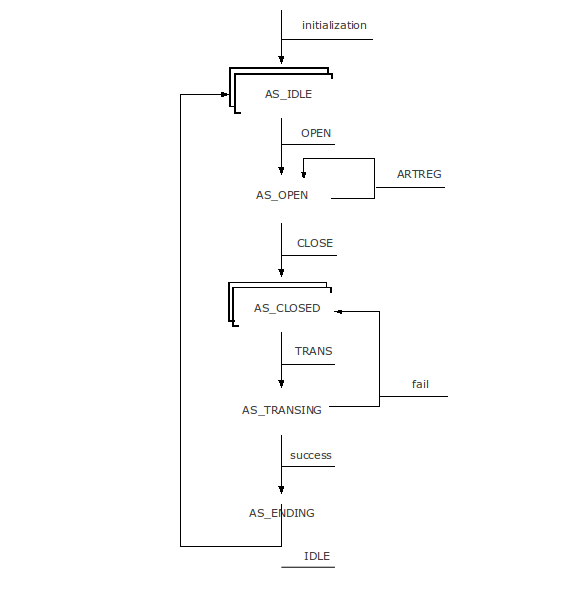
\includegraphics[width=0.6\textwidth]{account_lifecycle.png}
  \end{center}
  \caption{Registration Account State Machine}
  \label{fig:account-lifecycle}
\end{figure}

\section*{General Responses}
The following responses can, when appropriate, be generated as a response on any command. 
\vspace{5px} \\
\begin{tabular}{| l | p{280px} |}
\hline
500 Unknown command & In case the command is not recognized. \\ \hline
501 Syntax error & In case the command contains a syntax error  (e.g. mandatory argument is missing). \\ \hline
502 Command failed & As a last resort, when no other appropriate response can be given. \\ \hline
503 Error state & In case the CR is in Error state and the requested command cannot be processed due to that. \\ \hline
504 Weighing not available & This response should be used in the case a Cash register has a scale configured, but no connection between the Cash register and the scale is established, the Cash register must go to an error state and send a 504 error (weighing not available). \\ \hline
550 Not signed on & If the CR requires to be signed on for the command involved. \\ 
\hline
\end{tabular}

\section*{Commands}

\subsubsection*{Initialize SCRP Service}
\begin{tabular}{lp{350px}}
Command: & None; a transport connection suffices. \\
Description: & Initializes the SCRP service on the CR. The SFU must synchronize to the CR after the connection has been established. \\
Responses: & 220 SCRP Service ready \\
\end{tabular}

\subsubsection*{Terminate SCRP Service}
\begin{tabular}{lp{350px}}
Command: & QUIT \\
Description: & Requests the CR to smoothly terminate the SCRP service. Although the SFU should wait for all accounts to be AS\_IDLE before issuing this request, the CR must honour it in any state. Any non-IDLE account will be processed by the CR in an implementation defined manner. The CR remains ready to accept a (new) SFU connection. \\
Responses: & 221 SCRP Service terminating
\end{tabular}

\subsubsection*{Cash Register Sign On}
\begin{tabular}{lp{350px}}
Command: & SIGNON <SFU\_id>[:<password>] \\
Description: & Requests the CR to sign on, making the actual signing state SS\_ON. The CR is allowed to reject the request if the current signing state is SS\_HALT. \\
Responses: & 251 Signed On  \\
& 450 Signing rejected \\
& 551 Authentication failed
\end{tabular}

\subsubsection*{Cash Register Sign Off}
\begin{tabular}{lp{350px}}
Command: & SIGNOFF \\
Description: & Requests the CR to sign off, making the actual signing state SS\_OFF or SS\_HALT. The CR is allowed to reject the request if not all accounts are in AS\_IDLE state. Otherwise, any non-IDLE account will be processed by the CR in an implementation defined manner. \\
Responses: & 250 Signed Off \\
& 450 Signing rejected
\end{tabular}

\subsubsection*{Get CR Variable}
\begin{tabular}{lp{350px}}
Command: & GET <cr\_variable> \\
Description: & Requests to get the value of a certain CR Variable. The CR must honour this request in any state of the system. Possible variables and their values are listed in Table 3. \\
Responses: & 210 <cr\_variable>:<cr\_value> \\
& 510 No such variable
\end{tabular}

\subsubsection*{Open Account}
\begin{tabular}{lp{350px}}
Command: & OPEN [<account>|<barcode>] \\
Description: & Opens an account for subsequent article registrations. The CR is requested to perform this action before registration of articles commences. If the CR implementation is such that the account state is ``default opened" after the previous payment sequence, the command may internally have no effect but a positive response is still required. A positive response must report the identity of the account opened. If <account> or <barcode> is specified (both may be used alternatively), the command requests to recall the associated stored account. The format of <barcode> is the same as used by the CR to produce a store/recall ticket. A preferred implementation of this command returns an account number that is identical to the requested <account> (or identical to the account number from which <barcode> was constructed). Returning another account number is discouraged but allowed. The newly opened account must be put in state AS\_OPEN and must inherit all account data from the account that is recalled, including the state specific context. \\
Responses: & 231 <account> Account opened \\
& 530 No such account \\
& 531 Invalid account state
\end{tabular}

\subsubsection*{Close Current Account}
\begin{tabular}{lp{350px}}
Command: & CLOSE \\
Description: & Closes the current account for further registration. The CR is requested to perform this action before a transaction sequence is initiated. A positive response must include the total amount involved. The response may be preceeded by a series of `display responses', explaining the calculation from the previous subtotal to the current endtotal (e.g. mix-match calculation results). \\
Responses: & \{ 212 <description>[:<price>[:<amount>]] \} \\
& 230 <endtotal> Account closed \\
& 531 Invalid account state
\end{tabular}

\subsubsection*{Request Article Identification}
\begin{tabular}{lp{350px}}
Command: & ARTID <barcode> \\
Description: & Requests identification of an article, with <barcode> representing its key. This command is not a request to register the article. The CR must honor this request in any account state. A positive response must be given by means of a 211 response or a 213 response, their usage is alternative, which means that is up to the CR to use one or the other to respond to a given ARTID command. However systems using the certified weighing capability of the Cash Register must use the 213 response. Compared to the 211 response, the 213 response allows the CR to provide a full-scale specification of the attributes that characterize an article. A detailed definition of these responses including the error responses, is given hereunder. The length of the responses may never be larger then 512 characters. \\
Responses: & 213
\end{tabular}
  
\subsubsection*{Request Article Registration}
\begin{tabular}{lp{350px}}
Command: & ARTREG [<barcode>[:<amount>]] \\
Description: & Requests registration of an article, with <barcode> representing its key and <amount> representing the amount of articles to register. This request is not issued before an account has been opened successfully. A positive response must consist of the following elements: <nr\_articles> Actual number of articles registered, <subtotal>  Actual subtotal of articles registered. The response must be preceded by a series of `display responses' with all data related to the registration of this article (e.g. linked articles, discounts, etc.). If <barcode> is omitted, the command requests the complete list (as a series of `display responses') of articles registered in the current account, which might be a recalled account. In case of a recalled account for which a partial payment was carried out on the originating (stored) account, the list of `display responses' must include descriptive lines explaining the results of the partial payment(s) done; all in consistence with the value and definition of subtotal. If <amount> is omitted, it will default to 1. \\
Responses: & \{ 212 <description>[:<price>[:<amount>]] \} \\
& 232 <nr\_articles>:<subtotal> Article registered \\
& 511 No such article \\
& 531 Invalid account state
\end{tabular}

\subsubsection*{Request Account Transaction}
\begin{tabular}{lp{350px}}
Command: & TRANS <tr\_method>>[:<amount>] \\
Description: & Requests transaction of the `oldest' account from repository state AS\_CLOSED. The account must be closed before the request can be honoured. For details regarding transaction methods. A negative response (failure) must include an indicator that specifies the cause of the failure. Table 8 lists an overview of possible failures for each transaction method. Both transaction method and failure indication must be represented as ASCII strings and interpreted in a case-insensitive manner. If <amount> is omitted, the actual endtotal is assumed implicitly. Otherwise, <amount> indicates the requested transaction amount. The format of the <amount> argument is identical to that of <price>. The semantics of <amount> in relation to transaction methods TM\_STORE and TM\_FLUSH is undefined; in case <amount> is specified for these transaction methods, the response must report Failure Indication FI\_AMOUNT (see table below). After a successful transaction, the remaining endtotal must be updated accordingly and in correspondence with the applicable exchange calculation rules that reside in the CR; this endtotal value is also returned in the (new) ``240"-response. The resulting endtotal is by definition equal to 0 if the transaction was successful and the <amount> argument was omitted, even for TM\_STORE and TM\_FLUSH.
Different from what is specified in the Account State Machine of Figure~\ref{fig:account-lifecycle} the account state remains AS\_CLOSED after a successful transaction while the resulting endtotal is unequal to 0. This allows for repeated/split TRANS requests. \\
Responses: & 240 Transaction succeeded \\
& 531 Invalid account state \\
& 540 No such transaction method \\
& 541 Busy transacting \\
& 542 <failure\_ind> Transaction failed
\end{tabular}

\subsubsection*{Print to Receipt (CR-Printing only)}
\begin{tabular}{lp{350px}}
Command: & PRINT <account>:<html\_text> \\
Description: & Requests the CR to print HTML-style data to the receipt of the specified account. \\
Responses: & 260 Data printed \\
& 530 No such account \\
& 531 Invalid account state  \\
& 560 CR-printing inactive
\end{tabular}

\subsubsection*{Query Receipt (SFU-Printing only)}
\begin{tabular}{lp{350px}}
Command: & RECEIPT  \\
Description: & Queries the CR to generate a multiline response with the entire receipt of the account currently in AS\_ENDING state. \\
Responses: & \{ 261 <html\_text> \} \\
& 531 Invalid account state \\
& 561 SFU-printing inactive
\end{tabular}

\subsubsection*{Round-up Account}
\begin{tabular}{lp{350px}}
Command: & IDLE \\
Description: & Requests rounding-up of the account in AS\_ENDING state. A successful response makes the account state AS\_IDLE. In case of CR-printing, this command may cause he CR to activate the receipt cutter. With SFU-printing, this is the acknowledge to the CR that the receipt has been correctly printed. \\
Responses: & 233 Account idled \\
& 531 Invalid account state
\end{tabular}

\subsubsection*{Resume Operation}
\begin{tabular}{lp{350px}}
Command: & RESUME \\
Description: & Requests the CR to continue operation from Error state. Once the CR is in Error state, this command is needed to resume normal operation. \\
Responses: & 201 Resumed operation \\
& 503 Error state
\end{tabular}

\subsubsection*{Request Account EndTotal}
\begin{tabular}{lp{350px}}
Command: & ENDTOT \\
Description: & Requests to calculate the actual endtotal for the current account. The request is only valid in state AS\_OPEN. The response must be preceded by a series of `display responses', explaining the difference between the current subtotal and the calculated endtotal. As such, the responses to this command are similar to those of the ``CLOSE" command. In contrast with the ``CLOSE" command, ``ENDTOT" must not affect the account state and may be issued repeatedly. \\
Responses: & \{ 212 <description>[:<price>[:<amount>]] \} \\
& 230 <endtotal> Account endtotal \\
& 531 Invalid account state
\end{tabular}

\subsubsection*{Request print of Receipt Hardcopy}
\begin{tabular}{lp{350px}}
Command: & RHCOPY [<account>|<barcode>] \\
Description: & Requests the CR to print a hardcopy of a receipt. If <account> or <barcode> is omitted, requests to print a hardcopy of the last printed receipt. This function is mandatory. A preferred implementation, however, must also support the arguments <account> or <barcode> (both may be used alternatively), in which case the command requests to print a hardcopy of the receipt associated to the specified account. The format of <barcode> is syntactically the same as used by the CR to produce a store/recall ticket. It is preferred to accept this command in all/most account states recognized by the SCRP protocol. Accepting this command in account state AS\_IDLE is required, though. The receipt hardcopy must consist of all CR-generated print data for the designated account, as well as all data that was PRINT-ed for that account on behalf of the SFU. \\
Responses: & 260 Data printed \\
& 530 No such account \\
& 531 Invalid account state \\
& 560 CR-printing inactive
\end{tabular}

\subsubsection*{Cash Register Reset}
\begin{tabular}{lp{350px}}
Command: & RESETCR \\
Description: & Requests the CR to execute a reset. The function will only be possible to execute manually from within the SFU. \\
Responses: & 202 Cash Register restored \\
& 531 Invalid account state
\end{tabular}

\subsubsection*{Certified Weighing}
\begin{tabular}{lp{350px}}
Command: & GET CERTDATA <barcode> \\
Description: & This command requests certified weight data from the CR to be presented on the screen for human verification. The format of <barcode> is missing the embedded weight or price information. The Command can only be issued during the state AS\_OPEN. \\
Responses: & 214 \\
& 512 No stable weight \\
& 531 Invalid account state
\end{tabular}

  \newpage
  \chapter{SCRP IOGG}\label{app:scrp-gg}
  This appendix gives the IOGG for the Scanflow Cash Register Protocol. The protocol is described in section~\ref{sec:scrp}. Each figure groups together the rules for one aspect of the protocol. The captions under each rule give the stimulus or response it represents.
  \begin{figure}[ht]
\begin{center}
\subfloat[?ARTREG\_EXIST]{% To use this figure in your LaTeX document
% import the package groove/resources/groove2tikz.sty
%
% Special colors
\begin{tikzpicture}[
% Special color styles
scale=\tikzscale]
\node[newnode] (n2)  at (1.975, -0.410) {\ml{\textbf{Request}\\\textit{artreg\_exist}}};
\node[node] (n0)  at (0.850, -1.155) {\ml{\textbf{CR}}};
\node[node] (n1)  at (3.180, -1.145) {\ml{\textbf{SFU}}};
\node[nacnode] (n3)  at (2.005, -1.835) {\ml{\textbf{Request}}};
\path[newedge] (n2)  -- node[newlab]{to} (n0) ;
\path[nacedge] (n1)  -- node[naclab]{from} (n3) ;
\path[nacedge] (n3)  -- node[naclab]{to} (n0) ;
\path[edge](n0.east |- 3.180, -1.145) -- node[lab]{connection} (n1) ;
\path[newedge] (n1)  -- node[newlab]{from} (n2) ;
\userdefinedmacro
\end{tikzpicture}
\renewcommand{\userdefinedmacro}{\relax}
}\hspace{20px}
\subfloat[?ARTREG\_NEXIST]{% To use this figure in your LaTeX document
% import the package groove/resources/groove2tikz.sty
%
% Special colors
\begin{tikzpicture}[
% Special color styles
scale=\tikzscale]
\node[nacnode] (n3)  at (2.005, -1.835) {\ml{\textbf{Request}}};
\node[node] (n1)  at (3.180, -1.145) {\ml{\textbf{SFU}}};
\node[node] (n0)  at (0.850, -1.155) {\ml{\textbf{CR}}};
\node[newnode] (n2)  at (1.975, -0.410) {\ml{\textbf{Request}\\\textit{artreg\_nexist}}};
\path[newedge] (n2)  -- node[newlab]{to} (n0) ;
\path[nacedge] (n1)  -- node[naclab]{from} (n3) ;
\path[nacedge] (n3)  -- node[naclab]{to} (n0) ;
\path[edge](n0.east |- 3.180, -1.145) -- node[lab]{connection} (n1) ;
\path[newedge] (n1)  -- node[newlab]{from} (n2) ;
\userdefinedmacro
\end{tikzpicture}
\renewcommand{\userdefinedmacro}{\relax}
}\\
\subfloat[!212]{% To use this figure in your LaTeX document
% import the package groove/resources/groove2tikz.sty
%
% Special colors
\begin{tikzpicture}[
% Special color styles
scale=\tikzscale]
\node[node] (n3)  at (0.610, -1.600) {\ml{\textbf{Account}\\\textit{AS\_OPEN}}};
\node[node] (n1)  at (1.840, -1.605) {\ml{\textbf{SFU}}};
\node[node] (n0)  at (0.605, -0.870) {\ml{\textbf{CR}\\\textit{SS\_ON}}};
\node[node] (n2)  at (1.825, -0.900) {\ml{\textbf{Request}\\\textit{artreg\_exist}}};
\path[edge](n1.north -| 1.825, -0.900) -- node[lab]{from} (n2) ;
\path[edge](n2.west |- 0.605, -0.870) -- node[lab]{to} (n0) ;
\path[edge](n0.south -| 0.610, -1.600) -- node[lab]{has} (n3) ;
\userdefinedmacro
\end{tikzpicture}
\renewcommand{\userdefinedmacro}{\relax}
}\hspace{20px}
\subfloat[!531]{% To use this figure in your LaTeX document
% import the package groove/resources/groove2tikz.sty
%
% Special colors
\begin{tikzpicture}[
% Special color styles
scale=\tikzscale]
\node[nacnode] (n2)  at (0.850, -1.950) {\ml{\textbf{Account}\\\textit{AS\_OPEN}}};
\node[node] (n1)  at (2.510, -1.935) {\ml{\textbf{SFU}}};
\node[node] (n0)  at (0.825, -0.950) {\ml{\textbf{CR}\\\textit{SS\_ON}}};
\node[delnode] (n3)  at (2.515, -0.970) {\ml{\textbf{Request}\\\textit{?[artreg\_nexist,artreg\_exist]}}};
\path[deledge](n1.north -| 2.515, -0.970) -- node[dellab]{from} (n3) ;
\path[nacedge](n0.south -| 0.850, -1.950) -- node[naclab]{has} (n2) ;
\path[deledge](n3.west |- 0.825, -0.950) -- node[dellab]{to} (n0) ;
\userdefinedmacro
\end{tikzpicture}
\renewcommand{\userdefinedmacro}{\relax}
}\\
\subfloat[!511]{% To use this figure in your LaTeX document
% import the package groove/resources/groove2tikz.sty
%
% Special colors
\begin{tikzpicture}[
% Special color styles
scale=\tikzscale]
\node[node] (n1)  at (3.330, -0.885) {\ml{\textbf{SFU}}};
\node[node] (n0)  at (0.945, -0.890) {\ml{\textbf{CR}\\\textit{SS\_ON}}};
\node[delnode] (n2)  at (2.085, -0.890) {\ml{\textbf{Request}\\\textit{artreg\_nexist}}};
\path[deledge](n1.west |- 2.085, -0.890) -- node[dellab]{from} (n2) ;
\path[deledge](n2.west |- 0.945, -0.890) -- node[dellab]{to} (n0) ;
\userdefinedmacro
\end{tikzpicture}
\renewcommand{\userdefinedmacro}{\relax}
}\hspace{20px}
\subfloat[!232]{% To use this figure in your LaTeX document
% import the package groove/resources/groove2tikz.sty
%
% Special colors
\begin{tikzpicture}[
% Special color styles
scale=\tikzscale]
\node[delnode] (n2)  at (1.955, -0.810) {\ml{\textbf{Request}\\\textit{artreg\_exist}}};
\node[node] (n1)  at (3.270, -0.795) {\ml{\textbf{SFU}}};
\node[node] (n0)  at (0.915, -0.770) {\ml{\textbf{CR}\\\textit{SS\_ON}}};
\node[node] (n3)  at (0.900, -1.910) {\ml{\textbf{Account}\\\textit{AS\_OPEN}}};
\path[deledge](n2.west |- 0.915, -0.770) -- node[dellab]{to} (n0) ;
\path[edge](n0.south -| 0.900, -1.910) -- node[lab]{has} (n3) ;
\path[deledge](n1.west |- 1.955, -0.810) -- node[dellab]{from} (n2) ;
\userdefinedmacro
\end{tikzpicture}
\renewcommand{\userdefinedmacro}{\relax}
}
\caption{Account Article Registration}
\end{center}
\end{figure}

\newpage
\begin{figure}[ht]
\begin{center}
\subfloat[?ARTRET\_EXIST]{% To use this figure in your LaTeX document
% import the package groove/resources/groove2tikz.sty
%
% Special colors
\begin{tikzpicture}[
% Special color styles
scale=\tikzscale]
\node[nacnode] (n3)  at (2.005, -1.835) {\ml{\textbf{Request}}};
\node[node] (n1)  at (3.180, -1.145) {\ml{\textbf{SFU}}};
\node[node] (n0)  at (0.850, -1.155) {\ml{\textbf{CR}}};
\node[newnode] (n2)  at (1.975, -0.410) {\ml{\textbf{Request}\\\textit{artret\_exist}}};
\path[newedge] (n2)  -- node[newlab]{to} (n0) ;
\path[nacedge] (n1)  -- node[naclab]{from} (n3) ;
\path[edge](n0.east |- 3.180, -1.145) -- node[lab]{connection} (n1) ;
\path[nacedge] (n3)  -- node[naclab]{to} (n0) ;
\path[newedge] (n1)  -- node[newlab]{from} (n2) ;
\userdefinedmacro
\end{tikzpicture}
\renewcommand{\userdefinedmacro}{\relax}
}\hspace{20px}
\subfloat[?ARTRET\_NEXIST]{% To use this figure in your LaTeX document
% import the package groove/resources/groove2tikz.sty
%
% Special colors
\begin{tikzpicture}[
% Special color styles
scale=\tikzscale]
\node[newnode] (n2)  at (1.970, -0.410) {\ml{\textbf{Request}\\\textit{artret\_nexist}}};
\node[node] (n0)  at (0.850, -1.155) {\ml{\textbf{CR}}};
\node[node] (n1)  at (3.180, -1.145) {\ml{\textbf{SFU}}};
\node[nacnode] (n3)  at (2.005, -1.835) {\ml{\textbf{Request}}};
\path[newedge] (n2)  -- node[newlab]{to} (n0) ;
\path[nacedge] (n1)  -- node[naclab]{from} (n3) ;
\path[edge](n0.east |- 3.180, -1.145) -- node[lab]{connection} (n1) ;
\path[nacedge] (n3)  -- node[naclab]{to} (n0) ;
\path[newedge] (n1)  -- node[newlab]{from} (n2) ;
\userdefinedmacro
\end{tikzpicture}
\renewcommand{\userdefinedmacro}{\relax}
}\\
\subfloat[!212]{% To use this figure in your LaTeX document
% import the package groove/resources/groove2tikz.sty
%
% Special colors
\begin{tikzpicture}[
% Special color styles
scale=\tikzscale]
\node[node] (n3)  at (0.630, -1.790) {\ml{\textbf{Account}\\\textit{AS\_OPEN}}};
\node[node] (n1)  at (3.090, -0.895) {\ml{\textbf{SFU}}};
\node[node] (n0)  at (0.605, -0.870) {\ml{\textbf{CR}\\\textit{SS\_ON}}};
\node[node] (n2)  at (1.825, -0.900) {\ml{\textbf{Request}\\\textit{artret\_exist}}};
\path[edge](n2.west |- 0.605, -0.870) -- node[lab]{to} (n0) ;
\path[edge](n0.south -| 0.630, -1.790) -- node[lab]{has} (n3) ;
\path[edge](n1.west |- 1.825, -0.900) -- node[lab]{from} (n2) ;
\userdefinedmacro
\end{tikzpicture}
\renewcommand{\userdefinedmacro}{\relax}
}\hspace{20px}
\subfloat[!531]{% To use this figure in your LaTeX document
% import the package groove/resources/groove2tikz.sty
%
% Special colors
\begin{tikzpicture}[
% Special color styles
scale=\tikzscale]
\node[nacnode] (n2)  at (0.860, -1.760) {\ml{\textbf{Account}\\\textit{AS\_OPEN}}};
\node[node] (n1)  at (2.480, -1.695) {\ml{\textbf{SFU}}};
\node[node] (n0)  at (0.825, -0.950) {\ml{\textbf{CR}\\\textit{SS\_ON}}};
\node[delnode] (n3)  at (2.510, -0.970) {\ml{\textbf{Request}\\\textit{?[artret\_exist,artret\_nexist]}}};
\path[deledge](n1.north -| 2.510, -0.970) -- node[dellab]{from} (n3) ;
\path[nacedge](n0.south -| 0.860, -1.760) -- node[naclab]{has} (n2) ;
\path[deledge](n3.west |- 0.825, -0.950) -- node[dellab]{to} (n0) ;
\userdefinedmacro
\end{tikzpicture}
\renewcommand{\userdefinedmacro}{\relax}
}\\
\subfloat[!511]{% To use this figure in your LaTeX document
% import the package groove/resources/groove2tikz.sty
%
% Special colors
\begin{tikzpicture}[
% Special color styles
scale=\tikzscale]
\node[delnode] (n2)  at (1.890, -0.880) {\ml{\textbf{Request}\\\textit{artret\_nexist}}};
\node[node] (n0)  at (0.605, -0.870) {\ml{\textbf{CR}\\\textit{SS\_ON}}};
\node[node] (n1)  at (3.220, -0.895) {\ml{\textbf{SFU}}};
\path[deledge](n2.west |- 0.605, -0.870) -- node[dellab]{to} (n0) ;
\path[deledge](n1.west |- 1.890, -0.880) -- node[dellab]{from} (n2) ;
\userdefinedmacro
\end{tikzpicture}
\renewcommand{\userdefinedmacro}{\relax}
}\hspace{20px}
\subfloat[!511]{% To use this figure in your LaTeX document
% import the package groove/resources/groove2tikz.sty
%
% Special colors
\begin{tikzpicture}[
% Special color styles
scale=\tikzscale]
\node[node] (n3)  at (0.630, -1.790) {\ml{\textbf{Account}\\\textit{AS\_OPEN}}};
\node[node] (n1)  at (1.780, -1.775) {\ml{\textbf{SFU}}};
\node[node] (n0)  at (0.605, -0.870) {\ml{\textbf{CR}\\\textit{SS\_ON}}};
\node[delnode] (n2)  at (1.780, -0.890) {\ml{\textbf{Request}\\\textit{artret\_exist}}};
\path[deledge](n1.north -| 1.780, -0.890) -- node[dellab]{from} (n2) ;
\path[deledge](n2.west |- 0.605, -0.870) -- node[dellab]{to} (n0) ;
\path[edge](n0.south -| 0.630, -1.790) -- node[lab]{has} (n3) ;
\userdefinedmacro
\end{tikzpicture}
\renewcommand{\userdefinedmacro}{\relax}
}\\
\subfloat[!232]{% To use this figure in your LaTeX document
% import the package groove/resources/groove2tikz.sty
%
% Special colors
\begin{tikzpicture}[
% Special color styles
scale=\tikzscale]
\node[node] (n3)  at (0.910, -1.490) {\ml{\textbf{Account}\\\textit{AS\_OPEN}}};
\node[node] (n0)  at (0.915, -0.770) {\ml{\textbf{CR}\\\textit{SS\_ON}}};
\node[node] (n1)  at (2.040, -1.485) {\ml{\textbf{SFU}}};
\node[delnode] (n2)  at (2.020, -0.770) {\ml{\textbf{Request}\\\textit{artret\_exist}}};
\path[deledge](n1.north -| 2.020, -0.770) -- node[dellab]{from} (n2) ;
\path[deledge](n2.west |- 0.915, -0.770) -- node[dellab]{to} (n0) ;
\path[edge](n0.south -| 0.910, -1.490) -- node[lab]{has} (n3) ;
\userdefinedmacro
\end{tikzpicture}
\renewcommand{\userdefinedmacro}{\relax}
}
\caption{Account Article Return}
\end{center}
\end{figure}

\newpage
\begin{figure}[ht]
\begin{center}
\subfloat[?CLOSE]{% To use this figure in your LaTeX document
% import the package groove/resources/groove2tikz.sty
%
% Special colors
\begin{tikzpicture}[
% Special color styles
scale=\tikzscale]
\node[nacnode] (n1)  at (1.985, -2.145) {\ml{\textbf{Request}}};
\node[newnode] (n0)  at (2.005, -0.400) {\ml{\textbf{Request}\\\textit{close}}};
\node[node] (n2)  at (0.760, -1.205) {\ml{\textbf{CR}}};
\node[node] (n11)  at (3.310, -1.195) {\ml{\textbf{SFU}}};
\path[edge](n2.east |- 3.310, -1.195) -- node[lab]{connection} (n11) ;
\path[nacedge] (n1)  -- node[naclab]{to} (n2) ;
\path[nacedge] (n11)  -- node[naclab]{from} (n1) ;
\path[newedge] (n0)  -- node[newlab]{to} (n2) ;
\path[newedge] (n11)  -- node[newlab]{from} (n0) ;
\userdefinedmacro
\end{tikzpicture}
\renewcommand{\userdefinedmacro}{\relax}
}\hspace{20px}
\subfloat[!212]{% To use this figure in your LaTeX document
% import the package groove/resources/groove2tikz.sty
%
% Special colors
\begin{tikzpicture}[
% Special color styles
scale=\tikzscale]
\node[node] (n8)  at (1.695, -0.760) {\ml{\textbf{Request}\\\textit{close}}};
\node[node] (n0)  at (0.570, -1.610) {\ml{\textbf{Account}\\\textit{AS\_OPEN}}};
\node[node] (n5)  at (0.595, -0.770) {\ml{\textbf{CR}\\\textit{SS\_ON}}};
\node[node] (n6)  at (1.680, -1.585) {\ml{\textbf{SFU}}};
\path[edge](n6.north -| 1.695, -0.760) -- node[lab]{from} (n8) ;
\path[edge](n8.west |- 0.595, -0.770) -- node[lab]{to} (n5) ;
\path[edge](n5.south -| 0.570, -1.610) -- node[lab]{has} (n0) ;
\userdefinedmacro
\end{tikzpicture}
\renewcommand{\userdefinedmacro}{\relax}
}\\
\subfloat[!531]{% To use this figure in your LaTeX document
% import the package groove/resources/groove2tikz.sty
%
% Special colors
\begin{tikzpicture}[
% Special color styles
scale=\tikzscale]
\node[node] (n11)  at (2.060, -1.635) {\ml{\textbf{SFU}}};
\node[node] (n2)  at (1.000, -0.885) {\ml{\textbf{CR}\\\textit{SS\_ON}}};
\node[delnode] (n0)  at (2.075, -0.890) {\ml{\textbf{Request}\\\textit{close}}};
\node[nacnode] (n1)  at (1.010, -1.650) {\ml{\textbf{Account}\\\textit{AS\_OPEN}}};
\path[deledge](n0.west |- 1.000, -0.885) -- node[dellab]{to} (n2) ;
\path[nacedge](n2.south -| 1.010, -1.650) -- node[naclab]{has} (n1) ;
\path[deledge](n11.north -| 2.075, -0.890) -- node[dellab]{from} (n0) ;
\userdefinedmacro
\end{tikzpicture}
\renewcommand{\userdefinedmacro}{\relax}
}\hspace{20px}
\subfloat[!230]{% To use this figure in your LaTeX document
% import the package groove/resources/groove2tikz.sty
%
% Special colors
\begin{tikzpicture}[
% Special color styles
scale=\tikzscale]
\node[node] (n6)  at (2.820, -0.725) {\ml{\textbf{SFU}}};
\node[node] (n5)  at (0.595, -0.770) {\ml{\textbf{CR}\\\textit{SS\_ON}}};
\node[node] (n0)  at (0.605, -1.735) {\ml{\textbf{Account}\\{\color{\blue}\textit{$-$ AS\_OPEN}}\\{\color{\green}\textit{$+$ AS\_CLOSED}}}};
\node[delnode] (n8)  at (1.695, -0.760) {\ml{\textbf{Request}\\\textit{close}}};
\path[deledge](n6.west |- 1.695, -0.760) -- node[dellab]{from} (n8) ;
\path[deledge](n8.west |- 0.595, -0.770) -- node[dellab]{to} (n5) ;
\path[edge](n5.south -| 0.605, -1.735) -- node[lab]{has} (n0) ;
\userdefinedmacro
\end{tikzpicture}
\renewcommand{\userdefinedmacro}{\relax}
}
\caption{Account Close}
\end{center}
\end{figure}

\newpage
\begin{figure}[ht]
\begin{center}
\subfloat[?IDLE]{% To use this figure in your LaTeX document
% import the package groove/resources/groove2tikz.sty
%
% Special colors
\begin{tikzpicture}[
% Special color styles
scale=\tikzscale]
\node[node] (n11)  at (3.310, -1.195) {\ml{\textbf{SFU}}};
\node[node] (n2)  at (0.760, -1.205) {\ml{\textbf{CR}}};
\node[newnode] (n0)  at (2.005, -0.400) {\ml{\textbf{Request}\\\textit{idle}}};
\node[nacnode] (n1)  at (1.985, -2.145) {\ml{\textbf{Request}}};
\path[edge](n2.east |- 3.310, -1.195) -- node[lab]{connection} (n11) ;
\path[nacedge] (n1)  -- node[naclab]{to} (n2) ;
\path[newedge] (n0)  -- node[newlab]{to} (n2) ;
\path[nacedge] (n11)  -- node[naclab]{from} (n1) ;
\path[newedge] (n11)  -- node[newlab]{from} (n0) ;
\userdefinedmacro
\end{tikzpicture}
\renewcommand{\userdefinedmacro}{\relax}
}\hspace{20px}
\subfloat[!531]{% To use this figure in your LaTeX document
% import the package groove/resources/groove2tikz.sty
%
% Special colors
\begin{tikzpicture}[
% Special color styles
scale=\tikzscale]
\node[delnode] (n3)  at (2.345, -0.850) {\ml{\textbf{Request}\\\textit{idle}}};
\node[node] (n2)  at (2.350, -1.525) {\ml{\textbf{SFU}}};
\node[node] (n1)  at (1.080, -0.845) {\ml{\textbf{CR}\\\textit{SS\_ON}}};
\node[nacnode] (n0)  at (1.050, -1.610) {\ml{\textbf{Account}\\\textit{AS\_ENDING}}};
\path[deledge](n2.north -| 2.345, -0.850) -- node[dellab]{from} (n3) ;
\path[nacedge](n1.south -| 1.050, -1.610) -- node[naclab]{has} (n0) ;
\path[deledge](n3.west |- 1.080, -0.845) -- node[dellab]{to} (n1) ;
\userdefinedmacro
\end{tikzpicture}
\renewcommand{\userdefinedmacro}{\relax}
}\\
\subfloat[!233]{% To use this figure in your LaTeX document
% import the package groove/resources/groove2tikz.sty
%
% Special colors
\begin{tikzpicture}[
% Special color styles
scale=\tikzscale]
\node[delnode] (n3)  at (3.245, -0.830) {\ml{\textbf{Request}\\\textit{idle}}};
\node[node] (n2)  at (4.350, -0.795) {\ml{\textbf{SFU}}};
\node[node] (n1)  at (1.985, -0.830) {\ml{\textbf{CR}\\\textit{SS\_ON}}};
\node[node] (n0)  at (0.785, -0.855) {\ml{\textbf{Account}\\{\color{\blue}\textit{$-$ AS\_ENDING}}\\{\color{\green}\textit{$+$ AS\_IDLE}}}};
\path[deledge](n2.west |- 3.245, -0.830) -- node[dellab]{from} (n3) ;
\path[edge](n1.west |- 0.785, -0.855) -- node[lab]{has} (n0) ;
\path[deledge](n3.west |- 1.985, -0.830) -- node[dellab]{to} (n1) ;
\userdefinedmacro
\end{tikzpicture}
\renewcommand{\userdefinedmacro}{\relax}
}
\caption{Account Ending}
\end{center}
\end{figure}

\newpage
\begin{figure}[ht]
\begin{center}
\subfloat[?ENDTOT]{% To use this figure in your LaTeX document
% import the package groove/resources/groove2tikz.sty
%
% Special colors
\begin{tikzpicture}[
% Special color styles
scale=\tikzscale]
\node[node] (n2)  at (0.700, -1.185) {\ml{\textbf{CR}}};
\node[node] (n11)  at (3.150, -1.175) {\ml{\textbf{SFU}}};
\node[newnode] (n0)  at (1.925, -0.380) {\ml{\textbf{Request}\\\textit{endtot\_display}}};
\node[nacnode] (n1)  at (1.945, -2.185) {\ml{\textbf{Request}}};
\path[edge](n2.east |- 3.150, -1.175) -- node[lab]{connection} (n11) ;
\path[nacedge] (n1)  -- node[naclab]{to} (n2) ;
\path[newedge] (n0)  -- node[newlab]{to} (n2) ;
\path[nacedge] (n11)  -- node[naclab]{from} (n1) ;
\path[newedge] (n11)  -- node[newlab]{from} (n0) ;
\userdefinedmacro
\end{tikzpicture}
\renewcommand{\userdefinedmacro}{\relax}
}\hspace{20px}
\subfloat[!212]{% To use this figure in your LaTeX document
% import the package groove/resources/groove2tikz.sty
%
% Special colors
\begin{tikzpicture}[
% Special color styles
scale=\tikzscale]
\node[node] (n0)  at (2.240, -0.865) {\ml{\textbf{Request}\\{\color{\blue}\textit{$-$ ?[endtot\_display,endtot]}}\\{\color{\green}\textit{$+$ endtot}}}};
\node[node] (n11)  at (2.240, -1.635) {\ml{\textbf{SFU}}};
\node[node] (n1)  at (0.510, -1.680) {\ml{\textbf{Account}\\\textit{AS\_OPEN}}};
\node[node] (n2)  at (0.495, -0.880) {\ml{\textbf{CR}\\\textit{SS\_ON}}};
\path[edge](n0.west |- 0.495, -0.880) -- node[lab]{to} (n2) ;
\path[edge](n2.south -| 0.510, -1.680) -- node[lab]{has} (n1) ;
\path[edge](n11.north -| 2.240, -0.865) -- node[lab]{from} (n0) ;
\userdefinedmacro
\end{tikzpicture}
\renewcommand{\userdefinedmacro}{\relax}
}\\
\subfloat[!531]{% To use this figure in your LaTeX document
% import the package groove/resources/groove2tikz.sty
%
% Special colors
\begin{tikzpicture}[
% Special color styles
scale=\tikzscale]
\node[node] (n2)  at (1.000, -0.885) {\ml{\textbf{CR}\\\textit{SS\_ON}}};
\node[nacnode] (n1)  at (1.000, -1.630) {\ml{\textbf{Account}\\\textit{AS\_OPEN}}};
\node[node] (n11)  at (2.120, -1.525) {\ml{\textbf{SFU}}};
\node[delnode] (n0)  at (2.120, -0.880) {\ml{\textbf{Request}\\\textit{endtot\_display}}};
\path[deledge](n0.west |- 1.000, -0.885) -- node[dellab]{to} (n2) ;
\path[nacedge](n2.south -| 1.000, -1.630) -- node[naclab]{has} (n1) ;
\path[deledge](n11.north -| 2.120, -0.880) -- node[dellab]{from} (n0) ;
\userdefinedmacro
\end{tikzpicture}
\renewcommand{\userdefinedmacro}{\relax}
}\hspace{20px}
\subfloat[!230]{% To use this figure in your LaTeX document
% import the package groove/resources/groove2tikz.sty
%
% Special colors
\begin{tikzpicture}[
% Special color styles
scale=\tikzscale]
\node[node] (n2)  at (1.005, -0.890) {\ml{\textbf{CR}\\\textit{SS\_ON}}};
\node[node] (n1)  at (1.010, -1.570) {\ml{\textbf{Account}\\\textit{AS\_OPEN}}};
\node[node] (n11)  at (2.130, -1.545) {\ml{\textbf{SFU}}};
\node[delnode] (n0)  at (2.125, -0.880) {\ml{\textbf{Request}\\\textit{endtot}}};
\path[deledge](n0.west |- 1.005, -0.890) -- node[dellab]{to} (n2) ;
\path[edge](n2.south -| 1.010, -1.570) -- node[lab]{has} (n1) ;
\path[deledge](n11.north -| 2.125, -0.880) -- node[dellab]{from} (n0) ;
\userdefinedmacro
\end{tikzpicture}
\renewcommand{\userdefinedmacro}{\relax}
}
\caption{Account Endtotal}
\end{center}
\end{figure}

\newpage
\begin{figure}[ht]
\begin{center}
\subfloat[?OPEN]{% To use this figure in your LaTeX document
% import the package groove/resources/groove2tikz.sty
%
% Special colors
\begin{tikzpicture}[
% Special color styles
scale=\tikzscale]
\node[nacnode] (n1)  at (1.925, -1.555) {\ml{\textbf{Request}}};
\node[newnode] (n0)  at (1.915, -0.810) {\ml{\textbf{Request}\\\textit{open}}};
\node[node] (n2)  at (0.920, -1.125) {\ml{\textbf{CR}}};
\node[node] (n11)  at (2.970, -1.095) {\ml{\textbf{SFU}}};
\path[nacedge] (n1)  -- node[naclab]{to} (n2) ;
\path[newedge] (n0)  -- node[newlab]{to} (n2) ;
\path[nacedge] (n11)  -- node[naclab]{from} (n1) ;
\path[newedge] (n11)  -- node[newlab]{from} (n0) ;
\userdefinedmacro
\end{tikzpicture}
\renewcommand{\userdefinedmacro}{\relax}
}\hspace{20px}
\subfloat[?OPEN\_EXIST]{% To use this figure in your LaTeX document
% import the package groove/resources/groove2tikz.sty
%
% Special colors
\begin{tikzpicture}[
% Special color styles
scale=\tikzscale]
\node[node] (n11)  at (3.650, -1.115) {\ml{\textbf{SFU}}};
\node[node] (n2)  at (1.030, -1.110) {\ml{\textbf{CR}\\\textit{SS\_ON}\\stored\_account = true}};
\node[newnode] (n0)  at (2.300, -0.480) {\ml{\textbf{Request}\\\textit{open\_exist}}};
\node[nacnode] (n1)  at (2.335, -1.985) {\ml{\textbf{Request}}};
\node[node] (n3)  at (1.055, -1.930) {\ml{\textbf{Account}\\\textit{AS\_IDLE}}};
\path[nacedge] (n1)  -- node[naclab]{to} (n2) ;
\path[newedge] (n0)  -- node[newlab]{to} (n2) ;
\path[newedge] (n11)  -- node[newlab]{from} (n0) ;
\path[nacedge] (n11)  -- node[naclab]{from} (n1) ;
\path[edge](n2.south -| 1.055, -1.930) -- node[lab]{has} (n3) ;
\path[edge](n2.east |- 3.650, -1.115) -- node[lab]{connection} (n11) ;
\userdefinedmacro
\end{tikzpicture}
\renewcommand{\userdefinedmacro}{\relax}
}\\
\subfloat[?OPEN\_NEXIST]{% To use this figure in your LaTeX document
% import the package groove/resources/groove2tikz.sty
%
% Special colors
\begin{tikzpicture}[
% Special color styles
scale=\tikzscale]
\node[node] (n11)  at (3.230, -1.095) {\ml{\textbf{SFU}}};
\node[node] (n2)  at (0.610, -1.095) {\ml{\textbf{CR}}};
\node[newnode] (n0)  at (1.880, -0.460) {\ml{\textbf{Request}\\\textit{open\_nexist}}};
\node[nacnode] (n1)  at (1.915, -1.965) {\ml{\textbf{Request}}};
\node[node] (n3)  at (0.615, -1.900) {\ml{\textbf{Account}\\\textit{AS\_IDLE}}};
\path[nacedge] (n1)  -- node[naclab]{to} (n2) ;
\path[nacedge] (n11)  -- node[naclab]{from} (n1) ;
\path[newedge] (n0)  -- node[newlab]{to} (n2) ;
\path[edge](n2.east |- 3.230, -1.095) -- node[lab]{connection} (n11) ;
\path[newedge] (n11)  -- node[newlab]{from} (n0) ;
\path[edge](n2.south -| 0.615, -1.900) -- node[lab]{has} (n3) ;
\userdefinedmacro
\end{tikzpicture}
\renewcommand{\userdefinedmacro}{\relax}
}\hspace{20px}
\subfloat[!531]{% To use this figure in your LaTeX document
% import the package groove/resources/groove2tikz.sty
%
% Special colors
\begin{tikzpicture}[
% Special color styles
scale=\tikzscale]
\node[delnode] (n0)  at (2.005, -0.890) {\ml{\textbf{Request}\\\textit{open}}};
\node[node] (n11)  at (3.070, -0.875) {\ml{\textbf{SFU}}};
\node[nacnode] (n1)  at (1.010, -1.940) {\ml{\textbf{Account}\\\textit{AS\_IDLE}}};
\node[node] (n2)  at (0.990, -0.875) {\ml{\textbf{CR}\\\textit{SS\_ON}}};
\path[nacedge](n2.south -| 1.010, -1.940) -- node[naclab]{has} (n1) ;
\path[deledge](n11.west |- 2.005, -0.890) -- node[dellab]{from} (n0) ;
\path[deledge](n0.west |- 0.990, -0.875) -- node[dellab]{to} (n2) ;
\userdefinedmacro
\end{tikzpicture}
\renewcommand{\userdefinedmacro}{\relax}
}\\
\subfloat[!530]{% To use this figure in your LaTeX document
% import the package groove/resources/groove2tikz.sty
%
% Special colors
\begin{tikzpicture}[
% Special color styles
scale=\tikzscale]
\node[node] (n2)  at (1.570, -0.765) {\ml{\textbf{CR}\\\textit{SS\_ON}}};
\node[node] (n11)  at (4.110, -0.755) {\ml{\textbf{SFU}}};
\node[delnode] (n3)  at (2.850, -0.760) {\ml{\textbf{Request}\\\textit{open\_nexist}}};
\path[deledge](n3.west |- 1.570, -0.765) -- node[dellab]{to} (n2) ;
\path[deledge](n11.west |- 2.850, -0.760) -- node[dellab]{from} (n3) ;
\userdefinedmacro
\end{tikzpicture}
\renewcommand{\userdefinedmacro}{\relax}
}\hspace{20px}
\subfloat[!231]{% To use this figure in your LaTeX document
% import the package groove/resources/groove2tikz.sty
%
% Special colors
\begin{tikzpicture}[
% Special color styles
scale=\tikzscale]
\node[delnode] (n3)  at (2.855, -0.770) {\ml{\textbf{Request}\\\textit{open}}};
\node[node] (n11)  at (2.850, -1.475) {\ml{\textbf{SFU}}};
\node[node] (n0)  at (1.705, -1.645) {\ml{\textbf{Account}\\{\color{\blue}\textit{$-$ AS\_IDLE}}\\{\color{\green}\textit{$+$ AS\_OPEN}}}};
\node[node] (n2)  at (1.695, -0.770) {\ml{\textbf{CR}\\\textit{SS\_ON}}};
\path[edge](n2.south -| 1.705, -1.645) -- node[lab]{has} (n0) ;
\path[deledge](n3.west |- 1.695, -0.770) -- node[dellab]{to} (n2) ;
\path[deledge](n11.north -| 2.855, -0.770) -- node[dellab]{from} (n3) ;
\userdefinedmacro
\end{tikzpicture}
\renewcommand{\userdefinedmacro}{\relax}
}
\caption{Account Open}
\end{center}
\end{figure}

\newpage
\begin{figure}[ht]
\begin{center}
\subfloat[?STAMPREG]{% To use this figure in your LaTeX document
% import the package groove/resources/groove2tikz.sty
%
% Special colors
\begin{tikzpicture}[
% Special color styles
scale=\tikzscale]
\node[node, attr] (n4)  at (3.200, -0.395) {\ml{0}};
\node[parnode] (n4p)  at (n4.north west) {0};
\node[newnode] (n2)  at (1.970, -0.410) {\ml{\textbf{Request}\\\textit{stampreg\_start}}};
\node[node] (n0)  at (0.850, -1.155) {\ml{\textbf{CR}}};
\node[node] (n1)  at (3.180, -1.145) {\ml{\textbf{SFU}}};
\node[nacnode] (n3)  at (2.005, -1.835) {\ml{\textbf{Request}}};
\path[newedge] (n2)  -- node[newlab]{to} (n0) ;
\path[nacedge] (n1)  -- node[naclab]{from} (n3) ;
\path[nacedge] (n3)  -- node[naclab]{to} (n0) ;
\path[edge](n0.east |- 3.180, -1.145) -- node[lab]{connection} (n1) ;
\path[newedge] (n1)  -- node[newlab]{from} (n2) ;
\userdefinedmacro
\end{tikzpicture}
\renewcommand{\userdefinedmacro}{\relax}
}\hspace{20px}
\subfloat[!212]{% To use this figure in your LaTeX document
% import the package groove/resources/groove2tikz.sty
%
% Special colors
\begin{tikzpicture}[
% Special color styles
scale=\tikzscale]
\node[node] (n2)  at (2.455, -0.895) {\ml{\textbf{Request}\\{\color{\blue}\textit{$-$ ?[stampreg,stampreg\_start]}}\\{\color{\green}\textit{$+$ stampreg}}}};
\node[node] (n0)  at (0.605, -0.870) {\ml{\textbf{CR}\\\textit{SS\_ON}}};
\node[node] (n1)  at (2.450, -1.625) {\ml{\textbf{SFU}}};
\node[node] (n3)  at (0.630, -1.660) {\ml{\textbf{Account}\\\textit{AS\_CLOSED}}};
\path[edge](n1.north -| 2.455, -0.895) -- node[lab]{from} (n2) ;
\path[edge](n2.west |- 0.605, -0.870) -- node[lab]{to} (n0) ;
\path[edge](n0.south -| 0.630, -1.660) -- node[lab]{has} (n3) ;
\userdefinedmacro
\end{tikzpicture}
\renewcommand{\userdefinedmacro}{\relax}
}\\
\subfloat[!531]{% To use this figure in your LaTeX document
% import the package groove/resources/groove2tikz.sty
%
% Special colors
\begin{tikzpicture}[
% Special color styles
scale=\tikzscale]
\node[delnode] (n3)  at (2.165, -0.950) {\ml{\textbf{Request}\\\textit{stampreg\_start}}};
\node[node] (n0)  at (0.825, -0.950) {\ml{\textbf{CR}\\\textit{SS\_ON}}};
\node[node] (n1)  at (2.160, -1.625) {\ml{\textbf{SFU}}};
\node[nacnode] (n2)  at (0.810, -1.750) {\ml{\textbf{Account}\\\textit{AS\_CLOSED}}};
\path[deledge](n1.north -| 2.165, -0.950) -- node[dellab]{from} (n3) ;
\path[nacedge](n0.south -| 0.810, -1.750) -- node[naclab]{has} (n2) ;
\path[deledge](n3.west |- 0.825, -0.950) -- node[dellab]{to} (n0) ;
\userdefinedmacro
\end{tikzpicture}
\renewcommand{\userdefinedmacro}{\relax}
}\hspace{20px}
\subfloat[!511]{% To use this figure in your LaTeX document
% import the package groove/resources/groove2tikz.sty
%
% Special colors
\begin{tikzpicture}[
% Special color styles
scale=\tikzscale]
\node[node] (n1)  at (3.700, -0.895) {\ml{\textbf{SFU}}};
\node[node] (n0)  at (0.945, -0.890) {\ml{\textbf{CR}\\\textit{SS\_ON}}};
\node[delnode] (n2)  at (2.300, -0.890) {\ml{\textbf{Request}\\\textit{stampreg\_start}}};
\path[deledge](n2.west |- 0.945, -0.890) -- node[dellab]{to} (n0) ;
\path[deledge](n1.west |- 2.300, -0.890) -- node[dellab]{from} (n2) ;
\userdefinedmacro
\end{tikzpicture}
\renewcommand{\userdefinedmacro}{\relax}
}\\
\subfloat[!232]{% To use this figure in your LaTeX document
% import the package groove/resources/groove2tikz.sty
%
% Special colors
\begin{tikzpicture}[
% Special color styles
scale=\tikzscale]
\node[node] (n3)  at (0.900, -1.440) {\ml{\textbf{Account}\\\textit{AS\_CLOSED}}};
\node[node] (n0)  at (0.915, -0.770) {\ml{\textbf{CR}\\\textit{SS\_ON}}};
\node[node] (n1)  at (1.950, -1.425) {\ml{\textbf{SFU}}};
\node[delnode] (n2)  at (1.955, -0.810) {\ml{\textbf{Request}\\\textit{stampreg}}};
\path[deledge](n1.north -| 1.955, -0.810) -- node[dellab]{from} (n2) ;
\path[deledge](n2.west |- 0.915, -0.770) -- node[dellab]{to} (n0) ;
\path[edge](n0.south -| 0.900, -1.440) -- node[lab]{has} (n3) ;
\userdefinedmacro
\end{tikzpicture}
\renewcommand{\userdefinedmacro}{\relax}
}
\caption{Account Stamp Registration}
\end{center}
\end{figure}

\newpage
\begin{figure}[ht]
\begin{center}
\subfloat[?TRANS]{% To use this figure in your LaTeX document
% import the package groove/resources/groove2tikz.sty
%
% Special colors
\begin{tikzpicture}[
% Special color styles
scale=\tikzscale]
\node[node, attr] (n4)  at (2.825, -0.675) {\ml{"TM\_BANK"}};
\node[parnode] (n4p)  at (n4.north west) {0};
\node[nacnode] (n3)  at (1.335, -1.765) {\ml{\textbf{Request}}};
\node[newnode] (n2)  at (1.330, -0.580) {\ml{\textbf{Request}\\\textit{trans\_tm\_bank}}};
\node[node] (n0)  at (0.370, -1.225) {\ml{\textbf{CR}}};
\node[node] (n1)  at (2.140, -1.215) {\ml{\textbf{SFU}}};
\path[nacedge] (n1)  -- node[naclab]{from} (n3) ;
\path[edge](n0.east |- 2.140, -1.215) -- node[lab]{connection} (n1) ;
\path[newedge] (n1)  -- node[newlab]{from} (n2) ;
\path[newedge] (n2)  -- node[newlab]{to} (n0) ;
\path[nacedge] (n3)  -- node[naclab]{to} (n0) ;
\userdefinedmacro
\end{tikzpicture}
\renewcommand{\userdefinedmacro}{\relax}
}\hspace{20px}
\subfloat[?TRANS]{% To use this figure in your LaTeX document
% import the package groove/resources/groove2tikz.sty
%
% Special colors
\begin{tikzpicture}[
% Special color styles
scale=\tikzscale]
\node[node] (n1)  at (1.990, -1.245) {\ml{\textbf{SFU}}};
\node[node] (n0)  at (0.370, -1.225) {\ml{\textbf{CR}}};
\node[newnode] (n2)  at (1.185, -0.650) {\ml{\textbf{Request}\\\textit{trans\_tm\_cash}}};
\node[nacnode] (n3)  at (1.195, -1.815) {\ml{\textbf{Request}}};
\node[node, attr] (n4)  at (2.525, -0.735) {\ml{"TM\_CASH"}};
\node[parnode] (n4p)  at (n4.north west) {0};
\path[nacedge] (n1)  -- node[naclab]{from} (n3) ;
\path[edge](n0.east |- 1.990, -1.245) -- node[lab]{connection} (n1) ;
\path[newedge] (n1)  -- node[newlab]{from} (n2) ;
\path[newedge] (n2)  -- node[newlab]{to} (n0) ;
\path[nacedge] (n3)  -- node[naclab]{to} (n0) ;
\userdefinedmacro
\end{tikzpicture}
\renewcommand{\userdefinedmacro}{\relax}
}\\
\subfloat[?TRANS]{% To use this figure in your LaTeX document
% import the package groove/resources/groove2tikz.sty
%
% Special colors
\begin{tikzpicture}[
% Special color styles
scale=\tikzscale]
\node[node] (n1)  at (1.930, -1.235) {\ml{\textbf{SFU}}};
\node[node] (n0)  at (0.370, -1.225) {\ml{\textbf{CR}}};
\node[newnode] (n2)  at (1.155, -0.610) {\ml{\textbf{Request}\\\textit{trans\_tm\_store}}};
\node[nacnode] (n3)  at (1.145, -1.855) {\ml{\textbf{Request}}};
\node[node, attr] (n4)  at (2.505, -0.745) {\ml{"TM\_STORE"}};
\node[parnode] (n4p)  at (n4.north west) {0};
\path[nacedge] (n1)  -- node[naclab]{from} (n3) ;
\path[edge](n0.east |- 1.930, -1.235) -- node[lab]{connection} (n1) ;
\path[newedge] (n1)  -- node[newlab]{from} (n2) ;
\path[newedge] (n2)  -- node[newlab]{to} (n0) ;
\path[nacedge] (n3)  -- node[naclab]{to} (n0) ;
\userdefinedmacro
\end{tikzpicture}
\renewcommand{\userdefinedmacro}{\relax}
}\hspace{20px}
\subfloat[!531]{% To use this figure in your LaTeX document
% import the package groove/resources/groove2tikz.sty
%
% Special colors
\begin{tikzpicture}[
% Special color styles
scale=\tikzscale]
\node[delnode] (n3)  at (3.020, -0.600) {\ml{\textbf{Request}\\\textit{?[trans\_tm\_store,trans\_tm\_bank,trans\_tm\_cash]}}};
\node[nacnode] (n0)  at (0.690, -1.380) {\ml{\textbf{Account}\\\textit{AS\_CLOSED}}};
\node[node] (n1)  at (0.685, -0.590) {\ml{\textbf{CR}\\\textit{SS\_ON}}};
\node[node] (n2)  at (3.020, -1.255) {\ml{\textbf{SFU}}};
\path[deledge](n2.north -| 3.020, -0.600) -- node[dellab]{from} (n3) ;
\path[nacedge](n1.south -| 0.690, -1.380) -- node[naclab]{has} (n0) ;
\path[deledge](n3.west |- 0.685, -0.590) -- node[dellab]{to} (n1) ;
\userdefinedmacro
\end{tikzpicture}
\renewcommand{\userdefinedmacro}{\relax}
}\\
\subfloat[!240]{% To use this figure in your LaTeX document
% import the package groove/resources/groove2tikz.sty
%
% Special colors
\begin{tikzpicture}[
% Special color styles
scale=\tikzscale]
\node[delnode] (n10)  at (3.470, -0.490) {\ml{\textbf{Request}\\\textit{?[trans\_tm\_bank,trans\_tm\_cash]}}};
\node[node] (n0)  at (2.405, -1.385) {\ml{\textbf{Account}\\{\color{\blue}\textit{$-$ AS\_CLOSED}}\\{\color{\green}\textit{$+$ AS\_ENDING}}}};
\node[node] (n8)  at (1.195, -0.440) {\ml{\textbf{CR}\\\textit{SS\_ON}\\{\color{\green}$+$ stored\_account = false}}};
\node[node] (n9)  at (3.480, -1.205) {\ml{\textbf{SFU}}};
\node[node, attr] (n6)  at (1.150, -1.395) {\ml{\textbf{bool}}};
\path[deledge](n8.south -| 1.150, -1.395) -- node[dellab]{stored\_account} (n6) ;
\path[deledge](n10.west |- 1.195, -0.440) -- node[dellab]{to} (n8) ;
\path[edge] (n8)  -- node[lab]{has} (n0) ;
\path[deledge](n9.north -| 3.470, -0.490) -- node[dellab]{from} (n10) ;
\userdefinedmacro
\end{tikzpicture}
\renewcommand{\userdefinedmacro}{\relax}
}\hspace{20px}
\subfloat[!240]{% To use this figure in your LaTeX document
% import the package groove/resources/groove2tikz.sty
%
% Special colors
\begin{tikzpicture}[
% Special color styles
scale=\tikzscale]
\node[node, attr] (n6)  at (1.210, -1.335) {\ml{\textbf{bool}}};
\node[node] (n9)  at (3.690, -1.175) {\ml{\textbf{SFU}}};
\node[node] (n8)  at (1.695, -0.480) {\ml{\textbf{CR}\\\textit{SS\_ON}\\{\color{\green}$+$ stored\_account = true}}};
\node[node] (n0)  at (2.595, -1.305) {\ml{\textbf{Account}\\{\color{\blue}\textit{$-$ AS\_CLOSED}}\\{\color{\green}\textit{$+$ AS\_ENDING}}}};
\node[delnode] (n10)  at (3.480, -0.490) {\ml{\textbf{Request}\\\textit{trans\_tm\_store}}};
\path[deledge](n8.south -| 1.210, -1.335) -- node[dellab]{stored\_account} (n6) ;
\path[deledge](n10.west |- 1.695, -0.480) -- node[dellab]{to} (n8) ;
\path[edge] (n8)  -- node[lab]{has} (n0) ;
\path[deledge](n9.north -| 3.480, -0.490) -- node[dellab]{from} (n10) ;
\userdefinedmacro
\end{tikzpicture}
\renewcommand{\userdefinedmacro}{\relax}
}
\caption{Account Trans}
\end{center}
\end{figure}

\newpage
\begin{figure}[ht]
\begin{center}
\subfloat[?ARTID\_EXIST]{% To use this figure in your LaTeX document
% import the package groove/resources/groove2tikz.sty
%
% Special colors
\begin{tikzpicture}[
% Special color styles
scale=\tikzscale]
\node[nacnode] (n1)  at (1.945, -2.185) {\ml{\textbf{Request}}};
\node[newnode] (n0)  at (1.925, -0.380) {\ml{\textbf{Request}\\\textit{artid\_exist}}};
\node[node] (n11)  at (3.150, -1.175) {\ml{\textbf{SFU}}};
\node[node] (n2)  at (0.700, -1.185) {\ml{\textbf{CR}}};
\path[edge](n2.east |- 3.150, -1.175) -- node[lab]{connection} (n11) ;
\path[nacedge] (n1)  -- node[naclab]{to} (n2) ;
\path[nacedge] (n11)  -- node[naclab]{from} (n1) ;
\path[newedge] (n0)  -- node[newlab]{to} (n2) ;
\path[newedge] (n11)  -- node[newlab]{from} (n0) ;
\userdefinedmacro
\end{tikzpicture}
\renewcommand{\userdefinedmacro}{\relax}
}\hspace{20px}
\subfloat[?ARTID\_NEXIST]{% To use this figure in your LaTeX document
% import the package groove/resources/groove2tikz.sty
%
% Special colors
\begin{tikzpicture}[
% Special color styles
scale=\tikzscale]
\node[nacnode] (n1)  at (1.945, -2.185) {\ml{\textbf{Request}}};
\node[newnode] (n0)  at (1.925, -0.380) {\ml{\textbf{Request}\\\textit{artid\_nexist}}};
\node[node] (n11)  at (3.150, -1.175) {\ml{\textbf{SFU}}};
\node[node] (n2)  at (0.700, -1.185) {\ml{\textbf{CR}}};
\path[edge](n2.east |- 3.150, -1.175) -- node[lab]{connection} (n11) ;
\path[nacedge] (n1)  -- node[naclab]{to} (n2) ;
\path[newedge] (n0)  -- node[newlab]{to} (n2) ;
\path[nacedge] (n11)  -- node[naclab]{from} (n1) ;
\path[newedge] (n11)  -- node[newlab]{from} (n0) ;
\userdefinedmacro
\end{tikzpicture}
\renewcommand{\userdefinedmacro}{\relax}
}\\
\subfloat[!511]{% To use this figure in your LaTeX document
% import the package groove/resources/groove2tikz.sty
%
% Special colors
\begin{tikzpicture}[
% Special color styles
scale=\tikzscale]
\node[delnode] (n2)  at (2.175, -1.010) {\ml{\textbf{Request}\\\textit{artid\_nexist}}};
\node[node] (n1)  at (3.430, -0.995) {\ml{\textbf{SFU}}};
\node[node] (n0)  at (0.940, -1.005) {\ml{\textbf{CR}\\\textit{SS\_ON}}};
\path[deledge](n2.west |- 0.940, -1.005) -- node[dellab]{to} (n0) ;
\path[deledge](n1.west |- 2.175, -1.010) -- node[dellab]{from} (n2) ;
\userdefinedmacro
\end{tikzpicture}
\renewcommand{\userdefinedmacro}{\relax}
}\hspace{20px}
\subfloat[!213]{% To use this figure in your LaTeX document
% import the package groove/resources/groove2tikz.sty
%
% Special colors
\begin{tikzpicture}[
% Special color styles
scale=\tikzscale]
\node[delnode] (n2)  at (2.175, -1.010) {\ml{\textbf{Request}\\\textit{artid\_exist}}};
\node[node] (n1)  at (3.430, -0.995) {\ml{\textbf{SFU}}};
\node[node] (n0)  at (0.940, -1.005) {\ml{\textbf{CR}}};
\path[deledge](n2.west |- 0.940, -1.005) -- node[dellab]{to} (n0) ;
\path[deledge](n1.west |- 2.175, -1.010) -- node[dellab]{from} (n2) ;
\userdefinedmacro
\end{tikzpicture}
\renewcommand{\userdefinedmacro}{\relax}
}
\caption{Artid}
\end{center}
\end{figure}

\newpage
\begin{figure}[ht]
\begin{center}
\subfloat[!550]{% To use this figure in your LaTeX document
% import the package groove/resources/groove2tikz.sty
%
% Special colors
\begin{tikzpicture}[
% Special color styles
scale=\tikzscale]
\node[delnode] (n2)  at (2.185, -0.600) {\ml{\textbf{Request}\\{\color{\red}\textit{! signon}}}};
\node[node] (n1)  at (2.190, -1.235) {\ml{\textbf{SFU}}};
\node[node] (n0)  at (0.815, -0.610) {\ml{\textbf{CR}\\\textit{?[SS\_OFF,SS\_HALT]}}};
\path[deledge](n2.west |- 0.815, -0.610) -- node[dellab]{to} (n0) ;
\path[deledge](n1.north -| 2.185, -0.600) -- node[dellab]{from} (n2) ;
\userdefinedmacro
\end{tikzpicture}
\renewcommand{\userdefinedmacro}{\relax}
}\hspace{20px}
\subfloat[!501]{% To use this figure in your LaTeX document
% import the package groove/resources/groove2tikz.sty
%
% Special colors
\begin{tikzpicture}[
% Special color styles
scale=\tikzscale]
\node[node] (n0)  at (0.830, -0.560) {\ml{\textbf{CR}}};
\node[node] (n1)  at (3.130, -0.555) {\ml{\textbf{SFU}}};
\node[delnode] (n2)  at (1.815, -0.550) {\ml{\textbf{Request}\\\textit{resetcr}}};
\path[deledge](n2.west |- 0.830, -0.560) -- node[dellab]{to} (n0) ;
\path[deledge](n1.west |- 1.815, -0.550) -- node[dellab]{from} (n2) ;
\userdefinedmacro
\end{tikzpicture}
\renewcommand{\userdefinedmacro}{\relax}
}\\
\subfloat[!900]{% To use this figure in your LaTeX document
% import the package groove/resources/groove2tikz.sty
%
% Special colors
\begin{tikzpicture}[
% Special color styles
scale=\tikzscale]
\node[delnode] (n2)  at (1.735, -0.570) {\ml{\textbf{Request}\\\textit{?}}};
\node[node] (n1)  at (2.870, -0.565) {\ml{\textbf{SFU}}};
\node[node] (n0)  at (0.830, -0.555) {\ml{\textbf{CR}}};
\path[deledge](n2.west |- 0.830, -0.555) -- node[dellab]{to} (n0) ;
\path[deledge](n1.west |- 1.735, -0.570) -- node[dellab]{from} (n2) ;
\userdefinedmacro
\end{tikzpicture}
\renewcommand{\userdefinedmacro}{\relax}
}
\caption{General Responses}
\end{center}
\end{figure}

\newpage
\begin{figure}[ht]
\begin{center}
\subfloat[?GET]{% To use this figure in your LaTeX document
% import the package groove/resources/groove2tikz.sty
%
% Special colors
\begin{tikzpicture}[
% Special color styles
scale=\tikzscale]
\node[node, attr] (n5)  at (3.195, -1.875) {\ml{"CS\_SIGN"}};
\node[parnode] (n5p)  at (n5.north west) {0};
\node[node] (n2)  at (1.050, -1.175) {\ml{\textbf{CR}}};
\node[node] (n11)  at (3.220, -1.170) {\ml{\textbf{SFU}}};
\node[newnode] (n0)  at (1.965, -0.600) {\ml{\textbf{Request}\\\textit{get}}};
\node[nacnode] (n1)  at (1.945, -1.845) {\ml{\textbf{Request}}};
\node[node, attr] (n4)  at (3.205, -0.495) {\ml{\textbf{string}}};
\path[nacedge] (n1)  -- node[naclab]{to} (n2) ;
\path[edge](n2.east |- 3.220, -1.170) -- node[lab]{connection} (n11) ;
\path[newedge](n11.south -| 3.195, -1.875) -- node[newlab]{var\_name} (n5) ;
\path[newedge] (n0)  -- node[newlab]{to} (n2) ;
\path[nacedge] (n11)  -- node[naclab]{from} (n1) ;
\path[deledge](n11.north -| 3.205, -0.495) -- node[dellab]{var\_name} (n4) ;
\path[newedge] (n11)  -- node[newlab]{from} (n0) ;
\userdefinedmacro
\end{tikzpicture}
\renewcommand{\userdefinedmacro}{\relax}
}\hspace{20px}
\subfloat[?GET]{% To use this figure in your LaTeX document
% import the package groove/resources/groove2tikz.sty
%
% Special colors
\begin{tikzpicture}[
% Special color styles
scale=\tikzscale]
\node[node, attr] (n5)  at (3.195, -1.875) {\ml{"CS\_EVENT"}};
\node[parnode] (n5p)  at (n5.north west) {0};
\node[node] (n2)  at (1.050, -1.175) {\ml{\textbf{CR}}};
\node[node] (n11)  at (3.220, -1.170) {\ml{\textbf{SFU}}};
\node[newnode] (n0)  at (1.965, -0.600) {\ml{\textbf{Request}\\\textit{get}}};
\node[nacnode] (n1)  at (1.945, -1.845) {\ml{\textbf{Request}}};
\node[node, attr] (n4)  at (3.205, -0.495) {\ml{\textbf{string}}};
\path[nacedge] (n1)  -- node[naclab]{to} (n2) ;
\path[edge](n2.east |- 3.220, -1.170) -- node[lab]{connection} (n11) ;
\path[newedge](n11.south -| 3.195, -1.875) -- node[newlab]{var\_name} (n5) ;
\path[newedge] (n0)  -- node[newlab]{to} (n2) ;
\path[nacedge] (n11)  -- node[naclab]{from} (n1) ;
\path[deledge](n11.north -| 3.205, -0.495) -- node[dellab]{var\_name} (n4) ;
\path[newedge] (n11)  -- node[newlab]{from} (n0) ;
\userdefinedmacro
\end{tikzpicture}
\renewcommand{\userdefinedmacro}{\relax}
}\\
\subfloat[?GET]{% To use this figure in your LaTeX document
% import the package groove/resources/groove2tikz.sty
%
% Special colors
\begin{tikzpicture}[
% Special color styles
scale=\tikzscale]
\node[node, attr] (n4)  at (3.205, -0.495) {\ml{\textbf{string}}};
\node[nacnode] (n1)  at (1.945, -1.845) {\ml{\textbf{Request}}};
\node[newnode] (n0)  at (1.965, -0.600) {\ml{\textbf{Request}\\\textit{get}}};
\node[node] (n11)  at (3.220, -1.170) {\ml{\textbf{SFU}}};
\node[node] (n2)  at (1.050, -1.175) {\ml{\textbf{CR}}};
\node[node, attr] (n5)  at (3.195, -1.875) {\ml{"Unknown"}};
\node[parnode] (n5p)  at (n5.north west) {0};
\path[nacedge] (n1)  -- node[naclab]{to} (n2) ;
\path[edge](n2.east |- 3.220, -1.170) -- node[lab]{connection} (n11) ;
\path[newedge](n11.south -| 3.195, -1.875) -- node[newlab]{var\_name} (n5) ;
\path[newedge] (n0)  -- node[newlab]{to} (n2) ;
\path[nacedge] (n11)  -- node[naclab]{from} (n1) ;
\path[deledge](n11.north -| 3.205, -0.495) -- node[dellab]{var\_name} (n4) ;
\path[newedge] (n11)  -- node[newlab]{from} (n0) ;
\userdefinedmacro
\end{tikzpicture}
\renewcommand{\userdefinedmacro}{\relax}
}\hspace{20px}
\subfloat[!210]{% To use this figure in your LaTeX document
% import the package groove/resources/groove2tikz.sty
%
% Special colors
\begin{tikzpicture}[
% Special color styles
scale=\tikzscale]
\node[node, attr] (n3)  at (3.350, -1.730) {\ml{"CS\_SIGN"}};
\node[parnode] (n3p)  at (n3.north west) {0};
\node[delnode] (n2)  at (2.175, -1.010) {\ml{\textbf{Request}\\\textit{get}}};
\node[node] (n1)  at (3.330, -1.005) {\ml{\textbf{SFU}}};
\node[node] (n0)  at (0.950, -1.005) {\ml{\textbf{CR}}};
\node[node, attr] (n5)  at (0.960, -1.740) {\ml{\textbf{string}}};
\node[node, attr] (n4)  at (2.040, -1.740) {\ml{\textbf{string}}};
\node[parnode] (n4p)  at (n4.north west) {1};
\path[deledge](n1.west |- 2.175, -1.010) -- node[dellab]{from} (n2) ;
\path[deledge](n2.west |- 0.950, -1.005) -- node[dellab]{to} (n0) ;
\path[edge](n1.south -| 3.350, -1.730) -- node[lab]{var\_name} (n3) ;
\path[edge](n0.south -| 0.960, -1.740) -- node[lab]{state} (n5) ;
\path[edge, -](n5.east |- 2.040, -1.740) -- node[lab]{\textit{=}} (n4) ;
\userdefinedmacro
\end{tikzpicture}
\renewcommand{\userdefinedmacro}{\relax}
} \\
\subfloat[!210]{% To use this figure in your LaTeX document
% import the package groove/resources/groove2tikz.sty
%
% Special colors
\begin{tikzpicture}[
% Special color styles
scale=\tikzscale]
\node[node, prod] (n11)  at (3.050, -1.330) {\ml{or = true}};
\node[node, attr] (n10)  at (3.950, -1.640) {\ml{\textbf{bool}}};
\node[node, prod] (n9)  at (5.290, -1.650) {\ml{$\pi$1 = "EV\_NONE"}};
\node[node, attr] (n8)  at (3.950, -1.080) {\ml{\textbf{bool}}};
\node[node, prod] (n5)  at (5.280, -1.080) {\ml{$\pi$1 = "EV\_INFO"}};
\node[node, attr] (n3)  at (0.680, -1.740) {\ml{"CS\_EVENT"}};
\node[parnode] (n3p)  at (n3.north west) {0};
\node[delnode] (n2)  at (2.175, -1.010) {\ml{\textbf{Request}\\\textit{get}}};
\node[node] (n1)  at (2.180, -1.705) {\ml{\textbf{SFU}}};
\node[node] (n0)  at (0.750, -1.005) {\ml{\textbf{CR}}};
\node[node, attr] (n4)  at (6.770, -1.400) {\ml{\textbf{string}}};
\node[parnode] (n4p)  at (n4.north west) {1};
\path[deledge](n1.north -| 2.175, -1.010) -- node[dellab]{from} (n2) ;
\path[deledge](n2.west |- 0.750, -1.005) -- node[dellab]{to} (n0) ;
\path[edge](n1.west |- 0.680, -1.740) -- node[lab]{var\_name} (n3) ;
\path[edge] (n5)  -- node[lab]{$\pi$0} (n4) ;
\path[edge] (n5)  -- node[lab]{eq} (n8) ;
\path[edge] (n9)  -- node[lab]{$\pi$0} (n4) ;
\path[edge] (n9)  -- node[lab]{eq} (n10) ;
\path[edge] (n11)  -- node[lab]{$\pi$0} (n8) ;
\path[edge] (n11)  -- node[lab]{$\pi$1} (n10) ;
\userdefinedmacro
\end{tikzpicture}
\renewcommand{\userdefinedmacro}{\relax}
}\hspace{20px}
\subfloat[!510]{% To use this figure in your LaTeX document
% import the package groove/resources/groove2tikz.sty
%
% Special colors
\begin{tikzpicture}[
% Special color styles
scale=\tikzscale]
\node[delnode] (n2)  at (2.175, -1.010) {\ml{\textbf{Request}\\\textit{get}}};
\node[node] (n1)  at (2.170, -1.695) {\ml{\textbf{SFU}\\var\_name = "Unknown"}};
\node[node] (n0)  at (0.950, -1.005) {\ml{\textbf{CR}}};
\path[deledge](n1.north -| 2.175, -1.010) -- node[dellab]{from} (n2) ;
\path[deledge](n2.west |- 0.950, -1.005) -- node[dellab]{to} (n0) ;
\userdefinedmacro
\end{tikzpicture}
\renewcommand{\userdefinedmacro}{\relax}
}\\
\caption{Get Variable}
\end{center}
\end{figure}

\newpage
\begin{figure}[ht]
\begin{center}
\subfloat[!220]{% To use this figure in your LaTeX document
% import the package groove/resources/groove2tikz.sty
%
% Special colors
\begin{tikzpicture}[
% Special color styles
scale=\tikzscale]
\node[node] (n1)  at (3.500, -0.515) {\ml{\textbf{SFU}}};
\node[node] (n0)  at (1.340, -0.590) {\ml{\textbf{CR}\\{\color{\green}\textit{$+$ SS\_OFF}}\\{\color{\green}$+$ stored\_account = false}}};
\node[node, attr] (n3)  at (0.980, -1.465) {\ml{\textbf{bool}}};
\path[newedge] (n0) .. controls (1.850, -1.030) and (2.930, -0.990) ..  (n1) ;
\node[newlab] at (2.423, -0.988){connection};
\path[deledge](n0.south -| 0.980, -1.465) -- node[dellab]{stored\_account} (n3) ;
\path[nacedge](n0.east |- 3.500, -0.515) -- node[naclab]{connection} (n1) ;
\userdefinedmacro
\end{tikzpicture}
\renewcommand{\userdefinedmacro}{\relax}
}\hspace{20px}
\subfloat[Initial graph]{% To use this figure in your LaTeX document
% import the package groove/resources/groove2tikz.sty
%
% Special colors
\begin{tikzpicture}[
% Special color styles
scale=\tikzscale]
\node[node] (n0)  at (1.020, -1.065) {\ml{\textbf{CR}\\\textit{SS\_OFF}\\\textit{var\_1}\\state = "SS\_OFF"}};
\node[node] (n1)  at (2.420, -1.065) {\ml{\textbf{SFU}\\\textit{var\_2}\\var\_name = ""}};
\node[node] (n2)  at (1.035, -1.960) {\ml{\textbf{Account}\\\textit{AS\_IDLE}}};
\path[edge](n0.south -| 1.035, -1.960) -- node[lab]{has} (n2) ;
\userdefinedmacro
\end{tikzpicture}
\renewcommand{\userdefinedmacro}{\relax}
}
\caption{Initialize}
\end{center}
\end{figure}

\newpage
\begin{figure}[ht]
\begin{center}
\subfloat[?PRINT\_EXIST]{% To use this figure in your LaTeX document
% import the package groove/resources/groove2tikz.sty
%
% Special colors
\begin{tikzpicture}[
% Special color styles
scale=\tikzscale]
\node[node] (n2)  at (1.040, -1.205) {\ml{\textbf{CR}\\stored\_account = true}};
\node[node] (n11)  at (3.490, -1.195) {\ml{\textbf{SFU}}};
\node[newnode] (n0)  at (2.265, -0.400) {\ml{\textbf{Request}\\\textit{print\_exist}}};
\node[nacnode] (n1)  at (2.285, -2.205) {\ml{\textbf{Request}}};
\path[edge](n2.east |- 3.490, -1.195) -- node[lab]{connection} (n11) ;
\path[nacedge] (n1)  -- node[naclab]{to} (n2) ;
\path[newedge] (n0)  -- node[newlab]{to} (n2) ;
\path[nacedge] (n11)  -- node[naclab]{from} (n1) ;
\path[newedge] (n11)  -- node[newlab]{from} (n0) ;
\userdefinedmacro
\end{tikzpicture}
\renewcommand{\userdefinedmacro}{\relax}
}\hspace{20px}
\subfloat[?PRINT\_NEXIST]{% To use this figure in your LaTeX document
% import the package groove/resources/groove2tikz.sty
%
% Special colors
\begin{tikzpicture}[
% Special color styles
scale=\tikzscale]
\node[node] (n2)  at (0.700, -1.185) {\ml{\textbf{CR}}};
\node[node] (n11)  at (3.150, -1.175) {\ml{\textbf{SFU}}};
\node[newnode] (n0)  at (1.925, -0.380) {\ml{\textbf{Request}\\\textit{print\_nexist}}};
\node[nacnode] (n1)  at (1.945, -2.185) {\ml{\textbf{Request}}};
\path[edge](n2.east |- 3.150, -1.175) -- node[lab]{connection} (n11) ;
\path[nacedge] (n1)  -- node[naclab]{to} (n2) ;
\path[nacedge] (n11)  -- node[naclab]{from} (n1) ;
\path[newedge] (n0)  -- node[newlab]{to} (n2) ;
\path[newedge] (n11)  -- node[newlab]{from} (n0) ;
\userdefinedmacro
\end{tikzpicture}
\renewcommand{\userdefinedmacro}{\relax}
}\\
\subfloat[!560]{% To use this figure in your LaTeX document
% import the package groove/resources/groove2tikz.sty
%
% Special colors
\begin{tikzpicture}[
% Special color styles
scale=\tikzscale]
\node[delnode] (n2)  at (2.675, -1.000) {\ml{\textbf{Request}\\\textit{?[print\_exist,print\_nexist]}}};
\node[node] (n1)  at (4.250, -1.005) {\ml{\textbf{SFU}}};
\node[node] (n0)  at (0.945, -1.000) {\ml{\textbf{CR}\\\textit{SS\_ON}}};
\path[deledge](n2.west |- 0.945, -1.000) -- node[dellab]{to} (n0) ;
\path[deledge](n1.west |- 2.675, -1.000) -- node[dellab]{from} (n2) ;
\userdefinedmacro
\end{tikzpicture}
\renewcommand{\userdefinedmacro}{\relax}
}\hspace{20px}
\subfloat[!531]{% To use this figure in your LaTeX document
% import the package groove/resources/groove2tikz.sty
%
% Special colors
\begin{tikzpicture}[
% Special color styles
scale=\tikzscale]
\node[delnode] (n2)  at (2.595, -0.980) {\ml{\textbf{Request}\\\textit{print\_exist}}};
\node[node] (n1)  at (3.730, -0.955) {\ml{\textbf{SFU}}};
\node[node] (n0)  at (1.485, -0.980) {\ml{\textbf{CR}\\\textit{SS\_OFF}}};
\path[deledge](n1.west |- 2.595, -0.980) -- node[dellab]{from} (n2) ;
\path[deledge](n2.west |- 1.485, -0.980) -- node[dellab]{to} (n0) ;
\userdefinedmacro
\end{tikzpicture}
\renewcommand{\userdefinedmacro}{\relax}
}\\
\subfloat[!530]{% To use this figure in your LaTeX document
% import the package groove/resources/groove2tikz.sty
%
% Special colors
\begin{tikzpicture}[
% Special color styles
scale=\tikzscale]
\node[delnode] (n2)  at (2.115, -1.000) {\ml{\textbf{Request}\\\textit{print\_nexist}}};
\node[node] (n1)  at (2.120, -1.635) {\ml{\textbf{SFU}}};
\node[node] (n0)  at (0.945, -1.000) {\ml{\textbf{CR}\\\textit{SS\_ON}}};
\node[node] (n3)  at (0.970, -1.680) {\ml{\textbf{Account}\\{\color{\red}\textit{! AS\_IDLE}}}};
\path[deledge](n1.north -| 2.115, -1.000) -- node[dellab]{from} (n2) ;
\path[deledge](n2.west |- 0.945, -1.000) -- node[dellab]{to} (n0) ;
\path[edge](n0.south -| 0.970, -1.680) -- node[lab]{has} (n3) ;
\userdefinedmacro
\end{tikzpicture}
\renewcommand{\userdefinedmacro}{\relax}
}\hspace{20px}
\subfloat[!260]{% To use this figure in your LaTeX document
% import the package groove/resources/groove2tikz.sty
%
% Special colors
\begin{tikzpicture}[
% Special color styles
scale=\tikzscale]
\node[node] (n0)  at (0.950, -1.005) {\ml{\textbf{CR}\\\textit{SS\_ON}}};
\node[node] (n1)  at (3.330, -1.005) {\ml{\textbf{SFU}}};
\node[delnode] (n2)  at (2.175, -1.010) {\ml{\textbf{Request}\\\textit{print\_exist}}};
\path[deledge](n2.west |- 0.950, -1.005) -- node[dellab]{to} (n0) ;
\path[deledge](n1.west |- 2.175, -1.010) -- node[dellab]{from} (n2) ;
\userdefinedmacro
\end{tikzpicture}
\renewcommand{\userdefinedmacro}{\relax}
}
\caption{Print}
\end{center}
\end{figure}

\newpage
\begin{figure}[ht]
\begin{center}
\subfloat[?RECEIPT]{% To use this figure in your LaTeX document
% import the package groove/resources/groove2tikz.sty
%
% Special colors
\begin{tikzpicture}[
% Special color styles
scale=\tikzscale]
\node[nacnode] (n1)  at (1.595, -2.765) {\ml{\textbf{Request}}};
\node[newnode] (n0)  at (1.575, -1.400) {\ml{\textbf{Request}\\\textit{receipt}}};
\node[node] (n11)  at (2.800, -2.035) {\ml{\textbf{SFU}}};
\node[node] (n2)  at (0.490, -2.065) {\ml{\textbf{CR}}};
\path[edge](n2.east |- 2.800, -2.035) -- node[lab]{connection} (n11) ;
\path[nacedge] (n11)  -- node[naclab]{from} (n1) ;
\path[newedge] (n0)  -- node[newlab]{to} (n2) ;
\path[newedge] (n11)  -- node[newlab]{from} (n0) ;
\path[nacedge] (n1)  -- node[naclab]{to} (n2) ;
\userdefinedmacro
\end{tikzpicture}
\renewcommand{\userdefinedmacro}{\relax}
}\hspace{20px}
\subfloat[!261]{% To use this figure in your LaTeX document
% import the package groove/resources/groove2tikz.sty
%
% Special colors
\begin{tikzpicture}[
% Special color styles
scale=\tikzscale]
\node[node] (n2)  at (2.165, -1.010) {\ml{\textbf{Request}\\\textit{receipt}}};
\node[node] (n1)  at (3.330, -1.005) {\ml{\textbf{SFU}}};
\node[node] (n0)  at (0.945, -1.000) {\ml{\textbf{CR}\\\textit{SS\_ON}}};
\node[node] (n3)  at (0.950, -2.060) {\ml{\textbf{Account}\\\textit{AS\_ENDING}}};
\path[edge](n2.west |- 0.945, -1.000) -- node[lab]{to} (n0) ;
\path[edge](n0.south -| 0.950, -2.060) -- node[lab]{has} (n3) ;
\path[edge](n1.west |- 2.165, -1.010) -- node[lab]{from} (n2) ;
\userdefinedmacro
\end{tikzpicture}
\renewcommand{\userdefinedmacro}{\relax}
}\\
\subfloat[!531]{% To use this figure in your LaTeX document
% import the package groove/resources/groove2tikz.sty
%
% Special colors
\begin{tikzpicture}[
% Special color styles
scale=\tikzscale]
\node[node] (n0)  at (0.940, -0.995) {\ml{\textbf{CR}\\\textit{SS\_ON}}};
\node[node] (n1)  at (3.330, -1.005) {\ml{\textbf{SFU}}};
\node[delnode] (n2)  at (2.165, -1.010) {\ml{\textbf{Request}\\\textit{receipt}}};
\node[nacnode] (n3)  at (0.920, -1.960) {\ml{\textbf{Account}\\\textit{AS\_ENDING}}};
\path[deledge](n2.west |- 0.940, -0.995) -- node[dellab]{to} (n0) ;
\path[nacedge](n0.south -| 0.920, -1.960) -- node[naclab]{has} (n3) ;
\path[deledge](n1.west |- 2.165, -1.010) -- node[dellab]{from} (n2) ;
\userdefinedmacro
\end{tikzpicture}
\renewcommand{\userdefinedmacro}{\relax}
}\hspace{20px}
\subfloat[!561]{% To use this figure in your LaTeX document
% import the package groove/resources/groove2tikz.sty
%
% Special colors
\begin{tikzpicture}[
% Special color styles
scale=\tikzscale]
\node[delnode] (n2)  at (2.165, -1.010) {\ml{\textbf{Request}\\\textit{receipt}}};
\node[node] (n1)  at (3.330, -1.005) {\ml{\textbf{SFU}}};
\node[node] (n0)  at (0.945, -1.000) {\ml{\textbf{CR}\\\textit{SS\_ON}}};
\node[node] (n3)  at (0.950, -2.060) {\ml{\textbf{Account}\\\textit{AS\_ENDING}}};
\path[deledge](n2.west |- 0.945, -1.000) -- node[dellab]{to} (n0) ;
\path[edge](n0.south -| 0.950, -2.060) -- node[lab]{has} (n3) ;
\path[deledge](n1.west |- 2.165, -1.010) -- node[dellab]{from} (n2) ;
\userdefinedmacro
\end{tikzpicture}
\renewcommand{\userdefinedmacro}{\relax}
}\\
\subfloat[!261]{% To use this figure in your LaTeX document
% import the package groove/resources/groove2tikz.sty
%
% Special colors
\begin{tikzpicture}[
% Special color styles
scale=\tikzscale]
\node[node] (n3)  at (0.950, -1.750) {\ml{\textbf{Account}\\\textit{AS\_ENDING}}};
\node[node] (n0)  at (0.945, -1.000) {\ml{\textbf{CR}\\\textit{SS\_ON}}};
\node[node] (n1)  at (2.180, -1.725) {\ml{\textbf{SFU}}};
\node[delnode] (n2)  at (2.170, -1.010) {\ml{\textbf{Request}\\\textit{receipt}}};
\path[deledge](n1.north -| 2.170, -1.010) -- node[dellab]{from} (n2) ;
\path[deledge](n2.west |- 0.945, -1.000) -- node[dellab]{to} (n0) ;
\path[edge](n0.south -| 0.950, -1.750) -- node[lab]{has} (n3) ;
\userdefinedmacro
\end{tikzpicture}
\renewcommand{\userdefinedmacro}{\relax}
}
\caption{Receipt}
\end{center}
\end{figure}

\newpage
\begin{figure}[ht]
\begin{center}
\subfloat[?RHCOPY\_EXIST]{% To use this figure in your LaTeX document
% import the package groove/resources/groove2tikz.sty
%
% Special colors
\begin{tikzpicture}[
% Special color styles
scale=\tikzscale]
\node[node] (n2)  at (1.030, -1.205) {\ml{\textbf{CR}\\stored\_account = true}};
\node[node] (n11)  at (3.480, -1.195) {\ml{\textbf{SFU}}};
\node[newnode] (n0)  at (2.250, -0.400) {\ml{\textbf{Request}\\\textit{rhcopy\_exist}}};
\node[nacnode] (n1)  at (2.275, -2.205) {\ml{\textbf{Request}}};
\path[edge](n2.east |- 3.480, -1.195) -- node[lab]{connection} (n11) ;
\path[nacedge] (n1)  -- node[naclab]{to} (n2) ;
\path[newedge] (n0)  -- node[newlab]{to} (n2) ;
\path[nacedge] (n11)  -- node[naclab]{from} (n1) ;
\path[newedge] (n11)  -- node[newlab]{from} (n0) ;
\userdefinedmacro
\end{tikzpicture}
\renewcommand{\userdefinedmacro}{\relax}
}\hspace{20px}
\subfloat[?RHCOPY\_NEXIST]{% To use this figure in your LaTeX document
% import the package groove/resources/groove2tikz.sty
%
% Special colors
\begin{tikzpicture}[
% Special color styles
scale=\tikzscale]
\node[node] (n2)  at (0.700, -1.185) {\ml{\textbf{CR}}};
\node[node] (n11)  at (3.150, -1.175) {\ml{\textbf{SFU}}};
\node[newnode] (n0)  at (1.920, -0.380) {\ml{\textbf{Request}\\\textit{rhcopy\_nexist}}};
\node[nacnode] (n1)  at (1.945, -2.185) {\ml{\textbf{Request}}};
\path[edge](n2.east |- 3.150, -1.175) -- node[lab]{connection} (n11) ;
\path[nacedge] (n1)  -- node[naclab]{to} (n2) ;
\path[nacedge] (n11)  -- node[naclab]{from} (n1) ;
\path[newedge] (n0)  -- node[newlab]{to} (n2) ;
\path[newedge] (n11)  -- node[newlab]{from} (n0) ;
\userdefinedmacro
\end{tikzpicture}
\renewcommand{\userdefinedmacro}{\relax}
}\\
\subfloat[!560]{% To use this figure in your LaTeX document
% import the package groove/resources/groove2tikz.sty
%
% Special colors
\begin{tikzpicture}[
% Special color styles
scale=\tikzscale]
\node[delnode] (n2)  at (2.625, -1.000) {\ml{\textbf{Request}\\\textit{?[rhcopy\_exist,rhcopy\_nexist]}}};
\node[node] (n1)  at (4.330, -0.985) {\ml{\textbf{SFU}}};
\node[node] (n0)  at (0.945, -1.000) {\ml{\textbf{CR}\\\textit{SS\_ON}}};
\path[deledge](n2.west |- 0.945, -1.000) -- node[dellab]{to} (n0) ;
\path[deledge](n1.west |- 2.625, -1.000) -- node[dellab]{from} (n2) ;
\userdefinedmacro
\end{tikzpicture}
\renewcommand{\userdefinedmacro}{\relax}
}\hspace{20px}
\subfloat[!530]{% To use this figure in your LaTeX document
% import the package groove/resources/groove2tikz.sty
%
% Special colors
\begin{tikzpicture}[
% Special color styles
scale=\tikzscale]
\node[node] (n0)  at (0.940, -0.995) {\ml{\textbf{CR}\\\textit{SS\_ON}}};
\node[node] (n1)  at (3.330, -1.005) {\ml{\textbf{SFU}}};
\node[delnode] (n2)  at (2.170, -1.010) {\ml{\textbf{Request}\\\textit{rhcopy\_nexist}}};
\path[deledge](n2.west |- 0.940, -0.995) -- node[dellab]{to} (n0) ;
\path[deledge](n1.west |- 2.170, -1.010) -- node[dellab]{from} (n2) ;
\userdefinedmacro
\end{tikzpicture}
\renewcommand{\userdefinedmacro}{\relax}
}\\
\subfloat[!260]{% To use this figure in your LaTeX document
% import the package groove/resources/groove2tikz.sty
%
% Special colors
\begin{tikzpicture}[
% Special color styles
scale=\tikzscale]
\node[delnode] (n2)  at (2.170, -1.010) {\ml{\textbf{Request}\\\textit{rhcopy\_exist}}};
\node[node] (n1)  at (3.330, -1.005) {\ml{\textbf{SFU}}};
\node[node] (n0)  at (0.940, -0.995) {\ml{\textbf{CR}\\\textit{SS\_ON}}};
\node[node] (n3)  at (0.945, -2.055) {\ml{\textbf{Account}}};
\path[deledge](n2.west |- 0.940, -0.995) -- node[dellab]{to} (n0) ;
\path[edge](n0.south -| 0.945, -2.055) -- node[lab]{has} (n3) ;
\path[deledge](n1.west |- 2.170, -1.010) -- node[dellab]{from} (n2) ;
\userdefinedmacro
\end{tikzpicture}
\renewcommand{\userdefinedmacro}{\relax}
}
\caption{Receipt Hardcopy}
\end{center}
\end{figure}

\newpage
\begin{figure}[ht]
\begin{center}
\subfloat[?RESETCR]{% To use this figure in your LaTeX document
% import the package groove/resources/groove2tikz.sty
%
% Special colors
\begin{tikzpicture}[
% Special color styles
scale=\tikzscale]
\node[node] (n2)  at (0.700, -1.185) {\ml{\textbf{CR}}};
\node[node] (n11)  at (3.150, -1.175) {\ml{\textbf{SFU}}};
\node[newnode] (n0)  at (1.925, -0.380) {\ml{\textbf{Request}\\\textit{resetcr}}};
\node[nacnode] (n1)  at (1.945, -2.185) {\ml{\textbf{Request}}};
\path[edge](n2.east |- 3.150, -1.175) -- node[lab]{connection} (n11) ;
\path[nacedge] (n1)  -- node[naclab]{to} (n2) ;
\path[newedge] (n0)  -- node[newlab]{to} (n2) ;
\path[nacedge] (n11)  -- node[naclab]{from} (n1) ;
\path[newedge] (n11)  -- node[newlab]{from} (n0) ;
\userdefinedmacro
\end{tikzpicture}
\renewcommand{\userdefinedmacro}{\relax}
}\hspace{20px}
\subfloat[!531]{% To use this figure in your LaTeX document
% import the package groove/resources/groove2tikz.sty
%
% Special colors
\begin{tikzpicture}[
% Special color styles
scale=\tikzscale]
\node[node] (n0)  at (0.945, -1.000) {\ml{\textbf{CR}}};
\node[node] (n1)  at (3.330, -1.005) {\ml{\textbf{SFU}}};
\node[delnode] (n2)  at (2.175, -1.010) {\ml{\textbf{Request}\\\textit{resetcr}}};
\path[deledge](n2.west |- 0.945, -1.000) -- node[dellab]{to} (n0) ;
\path[deledge](n1.west |- 2.175, -1.010) -- node[dellab]{from} (n2) ;
\userdefinedmacro
\end{tikzpicture}
\renewcommand{\userdefinedmacro}{\relax}
}\\
\subfloat[!202]{% To use this figure in your LaTeX document
% import the package groove/resources/groove2tikz.sty
%
% Special colors
\begin{tikzpicture}[
% Special color styles
scale=\tikzscale]
\node[node] (n0)  at (0.940, -0.985) {\ml{\textbf{CR}}};
\node[node] (n1)  at (3.330, -1.005) {\ml{\textbf{SFU}}};
\node[delnode] (n2)  at (2.175, -1.010) {\ml{\textbf{Request}\\\textit{resetcr}}};
\path[deledge](n2.west |- 0.940, -0.985) -- node[dellab]{to} (n0) ;
\path[deledge](n1.west |- 2.175, -1.010) -- node[dellab]{from} (n2) ;
\userdefinedmacro
\end{tikzpicture}
\renewcommand{\userdefinedmacro}{\relax}
}
\caption{Resetcr}
\end{center}
\end{figure}

\newpage
\begin{figure}[ht]
\begin{center}
\subfloat[?SIGNOFF]{% To use this figure in your LaTeX document
% import the package groove/resources/groove2tikz.sty
%
% Special colors
\begin{tikzpicture}[
% Special color styles
scale=\tikzscale]
\node[nacnode] (n1)  at (1.945, -2.185) {\ml{\textbf{Request}}};
\node[newnode] (n0)  at (1.925, -0.380) {\ml{\textbf{Request}\\\textit{signoff}}};
\node[node] (n11)  at (3.150, -1.175) {\ml{\textbf{SFU}}};
\node[node] (n2)  at (0.700, -1.185) {\ml{\textbf{CR}}};
\path[edge](n2.east |- 3.150, -1.175) -- node[lab]{connection} (n11) ;
\path[nacedge] (n1)  -- node[naclab]{to} (n2) ;
\path[nacedge] (n11)  -- node[naclab]{from} (n1) ;
\path[newedge] (n0)  -- node[newlab]{to} (n2) ;
\path[newedge] (n11)  -- node[newlab]{from} (n0) ;
\userdefinedmacro
\end{tikzpicture}
\renewcommand{\userdefinedmacro}{\relax}
}\hspace{20px}
\subfloat[!450]{% To use this figure in your LaTeX document
% import the package groove/resources/groove2tikz.sty
%
% Special colors
\begin{tikzpicture}[
% Special color styles
scale=\tikzscale]
\node[node] (n6)  at (1.140, -1.530) {\ml{\textbf{Account}\\{\color{\red}\textit{! AS\_IDLE}}}};
\node[node] (n0)  at (1.135, -0.740) {\ml{\textbf{CR}\\\textit{SS\_ON}}};
\node[node] (n4)  at (2.380, -1.455) {\ml{\textbf{SFU}}};
\node[delnode] (n5)  at (2.395, -0.750) {\ml{\textbf{Request}\\\textit{signoff}}};
\path[edge](n0.south -| 1.140, -1.530) -- node[lab]{has} (n6) ;
\path[deledge](n5.west |- 1.135, -0.740) -- node[dellab]{to} (n0) ;
\path[deledge](n4.north -| 2.395, -0.750) -- node[dellab]{from} (n5) ;
\userdefinedmacro
\end{tikzpicture}
\renewcommand{\userdefinedmacro}{\relax}
}\\
\subfloat[!250]{% To use this figure in your LaTeX document
% import the package groove/resources/groove2tikz.sty
%
% Special colors
\begin{tikzpicture}[
% Special color styles
scale=\tikzscale]
\node[node] (n1)  at (4.360, -1.595) {\ml{\textbf{SFU}}};
\node[node] (n0)  at (1.160, -1.605) {\ml{\textbf{CR}\\{\color{\blue}\textit{$-$ ?[SS\_ON,SS\_OFF,SS\_HALT]}}\\{\color{\green}\textit{$+$ SS\_OFF}}}};
\node[delnode] (n2)  at (2.955, -1.600) {\ml{\textbf{Request}\\\textit{signoff}}};
\path[deledge](n2.west |- 1.160, -1.605) -- node[dellab]{to} (n0) ;
\path[deledge](n1.west |- 2.955, -1.600) -- node[dellab]{from} (n2) ;
\userdefinedmacro
\end{tikzpicture}
\renewcommand{\userdefinedmacro}{\relax}
}
\caption{Signoff}
\end{center}
\end{figure}

\newpage
\begin{figure}[ht]
\begin{center}
\subfloat[?SIGNON\_EXIST]{% To use this figure in your LaTeX document
% import the package groove/resources/groove2tikz.sty
%
% Special colors
\begin{tikzpicture}[
% Special color styles
scale=\tikzscale]
\node[node] (n11)  at (3.300, -1.155) {\ml{\textbf{SFU}}};
\node[node] (n2)  at (0.840, -1.165) {\ml{\textbf{CR}}};
\node[newnode] (n0)  at (2.045, -0.360) {\ml{\textbf{Request}\\\textit{signon\_exist}}};
\node[nacnode] (n1)  at (2.075, -2.095) {\ml{\textbf{Request}}};
\path[edge](n2.east |- 3.300, -1.155) -- node[lab]{connection} (n11) ;
\path[nacedge] (n1)  -- node[naclab]{to} (n2) ;
\path[newedge] (n0)  -- node[newlab]{to} (n2) ;
\path[nacedge] (n11)  -- node[naclab]{from} (n1) ;
\path[newedge] (n11)  -- node[newlab]{from} (n0) ;
\userdefinedmacro
\end{tikzpicture}
\renewcommand{\userdefinedmacro}{\relax}
}\hspace{20px}
\subfloat[?SIGNON\_NEXIST]{% To use this figure in your LaTeX document
% import the package groove/resources/groove2tikz.sty
%
% Special colors
\begin{tikzpicture}[
% Special color styles
scale=\tikzscale]
\node[nacnode] (n1)  at (2.075, -2.095) {\ml{\textbf{Request}}};
\node[newnode] (n0)  at (2.040, -0.360) {\ml{\textbf{Request}\\\textit{signon\_nexist}}};
\node[node] (n2)  at (0.840, -1.165) {\ml{\textbf{CR}}};
\node[node] (n11)  at (3.300, -1.155) {\ml{\textbf{SFU}}};
\path[edge](n2.east |- 3.300, -1.155) -- node[lab]{connection} (n11) ;
\path[nacedge] (n1)  -- node[naclab]{to} (n2) ;
\path[newedge] (n0)  -- node[newlab]{to} (n2) ;
\path[nacedge] (n11)  -- node[naclab]{from} (n1) ;
\path[newedge] (n11)  -- node[newlab]{from} (n0) ;
\userdefinedmacro
\end{tikzpicture}
\renewcommand{\userdefinedmacro}{\relax}
}\\
\subfloat[!551]{% To use this figure in your LaTeX document
% import the package groove/resources/groove2tikz.sty
%
% Special colors
\begin{tikzpicture}[
% Special color styles
scale=\tikzscale]
\node[delnode] (n2)  at (2.165, -0.700) {\ml{\textbf{Request}\\\textit{signon\_nexist}}};
\node[node] (n0)  at (1.040, -0.695) {\ml{\textbf{CR}}};
\node[node] (n1)  at (3.470, -0.675) {\ml{\textbf{SFU}}};
\path[deledge](n2.west |- 1.040, -0.695) -- node[dellab]{to} (n0) ;
\path[deledge](n1.west |- 2.165, -0.700) -- node[dellab]{from} (n2) ;
\userdefinedmacro
\end{tikzpicture}
\renewcommand{\userdefinedmacro}{\relax}
}\hspace{20px}
\subfloat[!450]{% To use this figure in your LaTeX document
% import the package groove/resources/groove2tikz.sty
%
% Special colors
\begin{tikzpicture}[
% Special color styles
scale=\tikzscale]
\node[node] (n1)  at (4.430, -0.735) {\ml{\textbf{SFU}}};
\node[node] (n0)  at (0.900, -0.775) {\ml{\textbf{CR}}};
\node[delnode] (n2)  at (2.550, -0.740) {\ml{\textbf{Request}\\\textit{?[signon\_exist,signon\_nexist]}}};
\path[deledge](n1.west |- 2.550, -0.740) -- node[dellab]{from} (n2) ;
\path[deledge](n2.west |- 0.900, -0.775) -- node[dellab]{to} (n0) ;
\userdefinedmacro
\end{tikzpicture}
\renewcommand{\userdefinedmacro}{\relax}
}\\
\subfloat[!251]{% To use this figure in your LaTeX document
% import the package groove/resources/groove2tikz.sty
%
% Special colors
\begin{tikzpicture}[
% Special color styles
scale=\tikzscale]
\node[node] (n1)  at (3.850, -0.705) {\ml{\textbf{SFU}}};
\node[node] (n0)  at (1.050, -0.705) {\ml{\textbf{CR}\\{\color{\blue}\textit{$-$ ?[SS\_OFF,SS\_HALT]}}\\{\color{\green}\textit{$+$ SS\_ON}}}};
\node[delnode] (n2)  at (2.555, -0.740) {\ml{\textbf{Request}\\\textit{signon\_exist}}};
\path[deledge](n2.west |- 1.050, -0.705) -- node[dellab]{to} (n0) ;
\path[deledge](n1.west |- 2.555, -0.740) -- node[dellab]{from} (n2) ;
\userdefinedmacro
\end{tikzpicture}
\renewcommand{\userdefinedmacro}{\relax}
}
\caption{Signon}
\end{center}
\end{figure}

